\setchapterpreamble[u]{\margintoc}
\chapter{Related Work}
\label{chapter-related-work}
\epigraph{I recall seeing a package to make quotes}{Snowball} % https://tex.stackexchange.com/a/53378/88466

% Additional, older material is online in https://docs.google.com/document/d/1OdoBsLboTZHzv1UP9g7nUriVLgpu6ZGqjXLmRAAlAfs/edit?usp=sharing
% New ideas and material are being added to a Google Doc for a while, then I'll revise this chapter. https://docs.google.com/document/d/1i3cCk2-8zwVioAuMbBQDLcUViihhHY6gk0MJNPevFbA/edit?usp=sharing

\begin{figure}
    \centering
    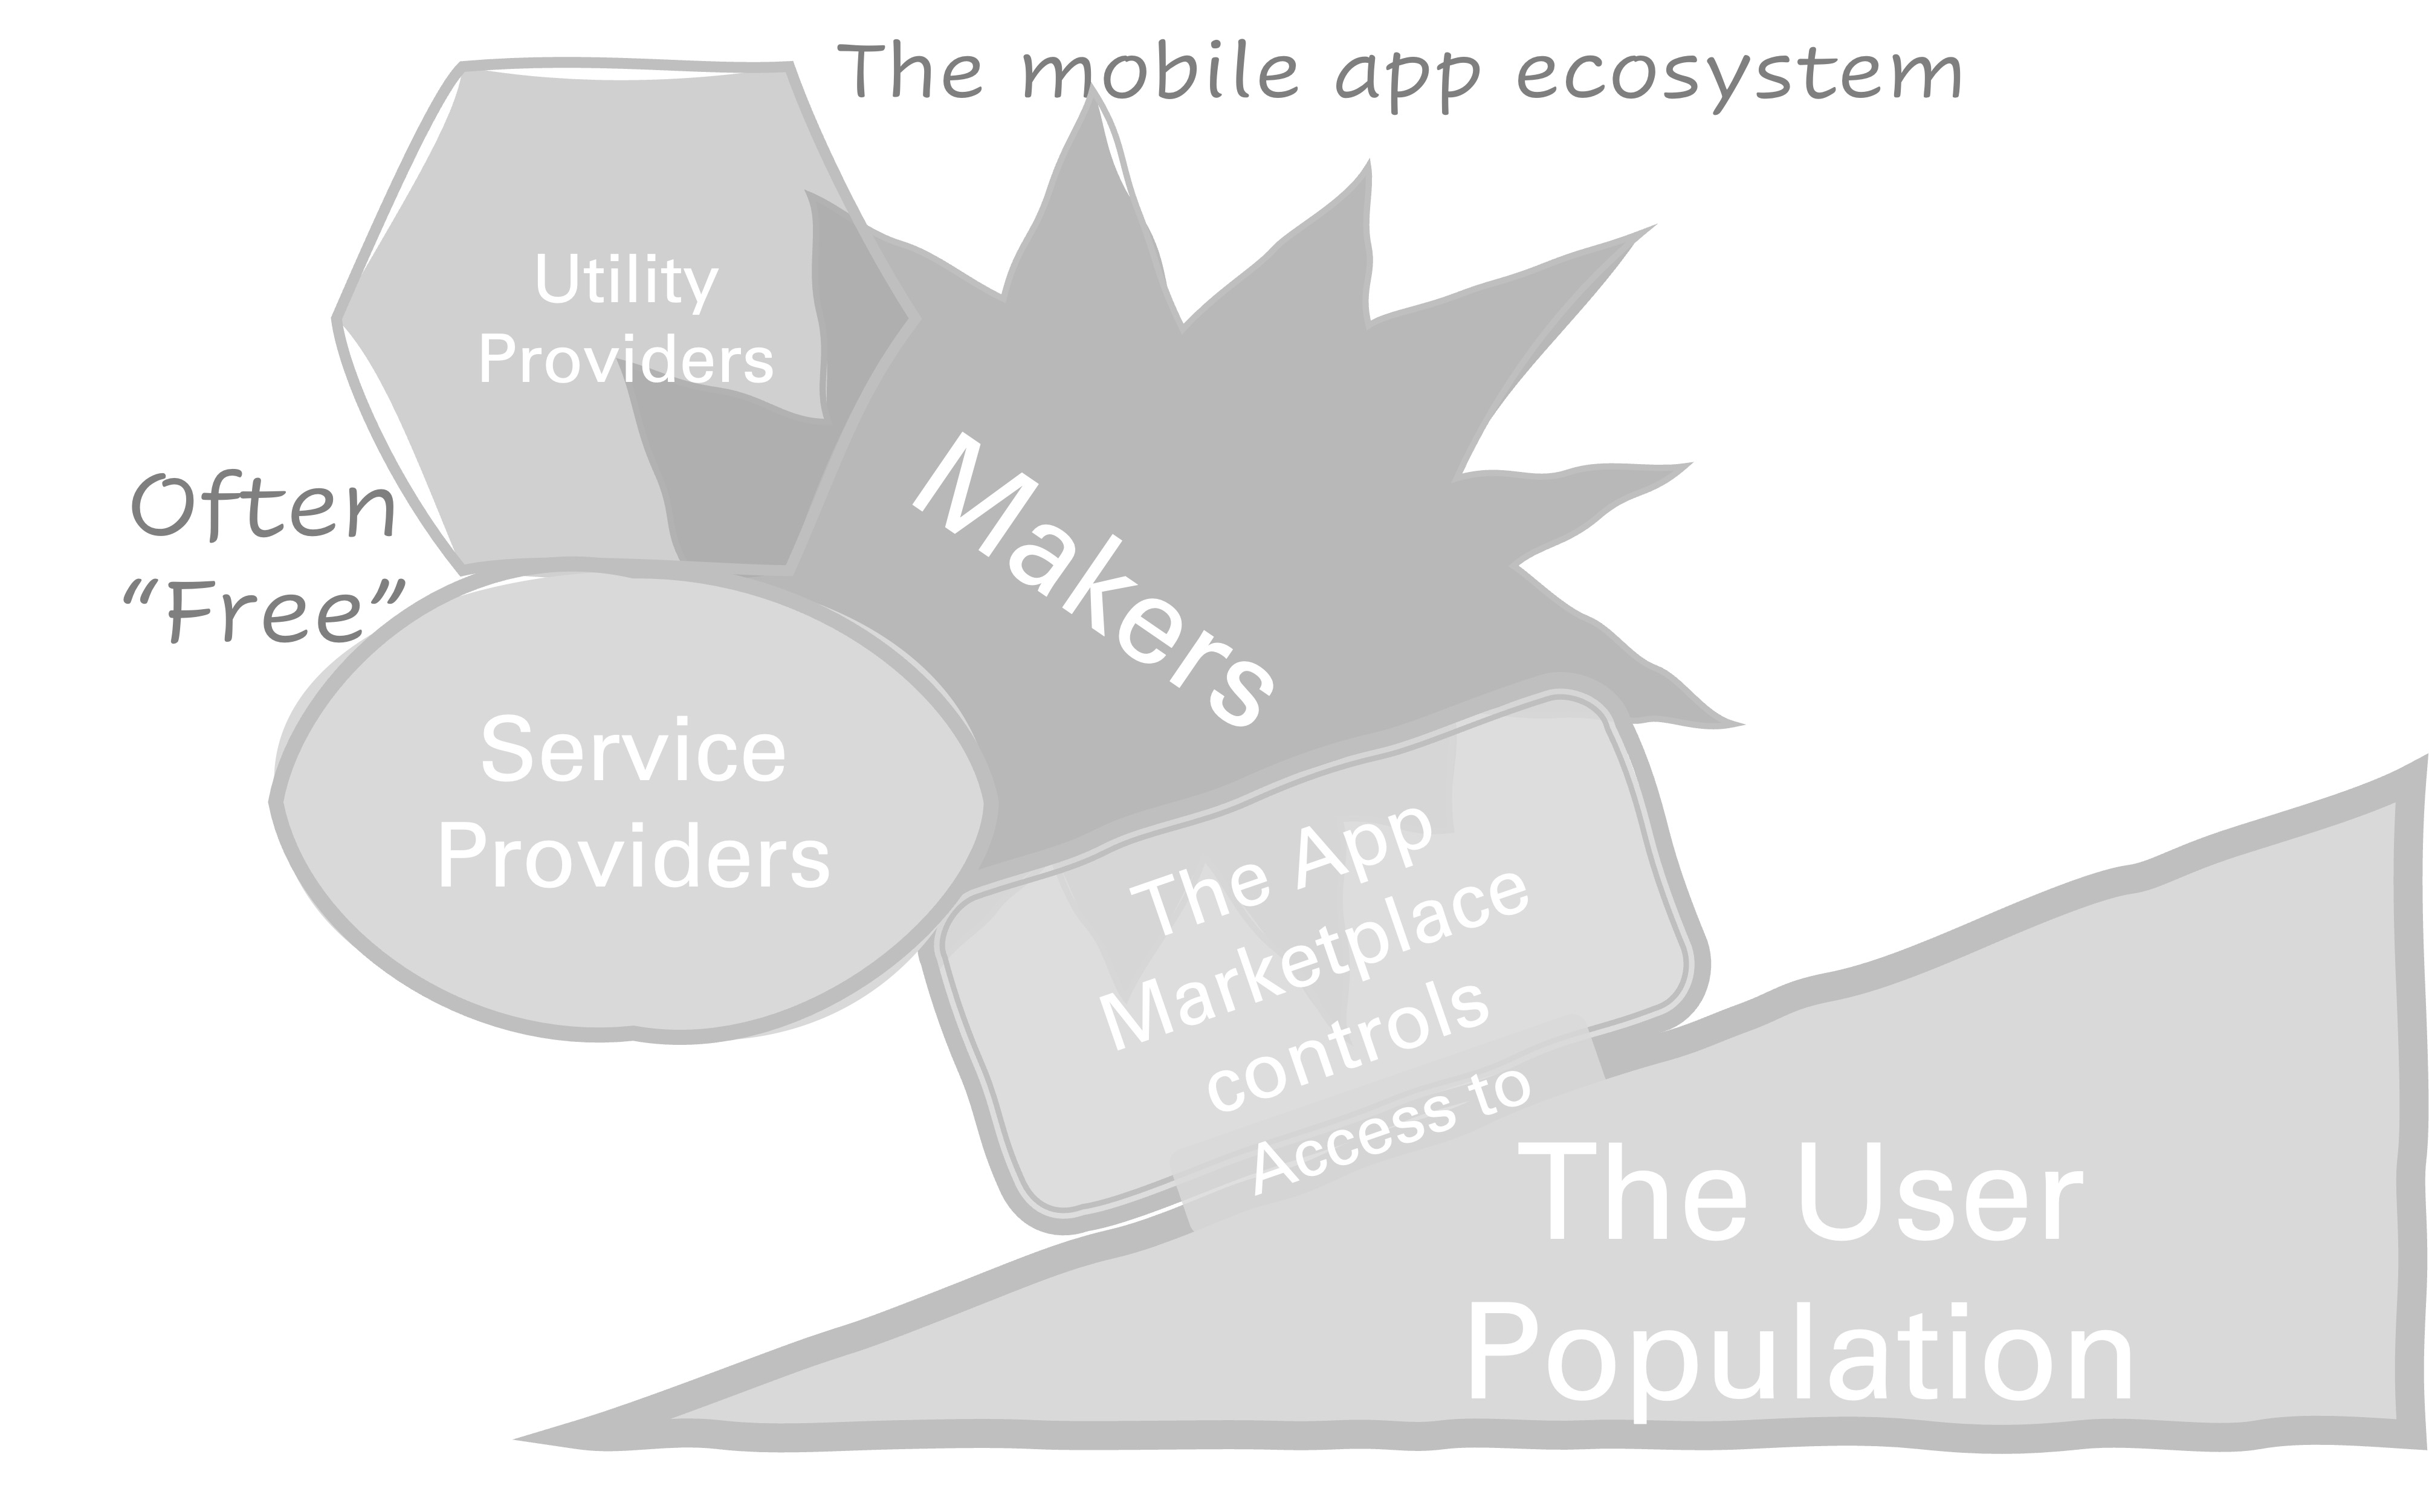
\includegraphics[width=\linewidth]{images/my/the-mobile-app-ecosystem-27-jul-2022.jpg}
    \caption{The Modern Mobile App Ecosystem}
    \label{fig:my_modern-mobile-app-ecosystem}
\end{figure}

The modern mobile ecosystem, illustrated in Figure~\ref{fig:my_modern-mobile-app-ecosystem}, 
sets the context for the thesis and this chapter together with the research questions. The marketplace - the app store - establishes the ecosystem which generates revenues from the user population and frequently to a lesser extent from the makers -  the developers of the apps. Various providers of utilities and services offer these to the makers and they may also obtain revenues from one or more parties that are part of the ecosystem and/or from others, including advertisers.

My work nestles within the works of many people in various related fields: in software quality, in analytics, and in the mobile device ecosystem. As researchers we understand and recognise there are gaps in the current state of the art, this chapter aims to identify several pertinent gaps which led to this research being performed, \emph{i.e.} which motivated me to act. The mobile ecosystems touch on billions of people's lives, where flaws in the apps and the ecosystem can adversely affect the lives of many of those people. 

Research in how mobile apps are created and tested, the relevance of app stores, service and utility providers, the user bases for mobile apps within the overall population of users of an app store ecosystem are all relevant. And meanwhile understanding why it's hard to create reliable software is also vital as part of acknowledging some of the grim realities development teams need to face if they are to succeed in their other goals and objectives for their mobile apps. An understanding of research into how to measure software qualities, and stability in particular, is key to establishing ways mobile analytics measures these qualities. 

At times this chapter will draw from broader sources, for instance in software development, testing, and analytics as these provide context for the particulars of the mobile app ecosystem. Conversely, in my view, and based on discussions at a peer workshop in Japan~\sidecite{nii_shonan_workshop_152}, I proposed a model, shown in Figure~\ref{fig:my_shonan_hysteresis_sketch}, that seemed to be well accepted and became part of the formal post-workshop report~\sidecite{nii_shonan_152_workshop_report}, where the mobile ecosystem is influencing the desktop app ecosystems. Examples include: app stores, per user licensing across multiple devices, public ratings and reviews, platform (device) level, crash reporting, and usage analytics, and so on.

\begin{figure}
    \centering
    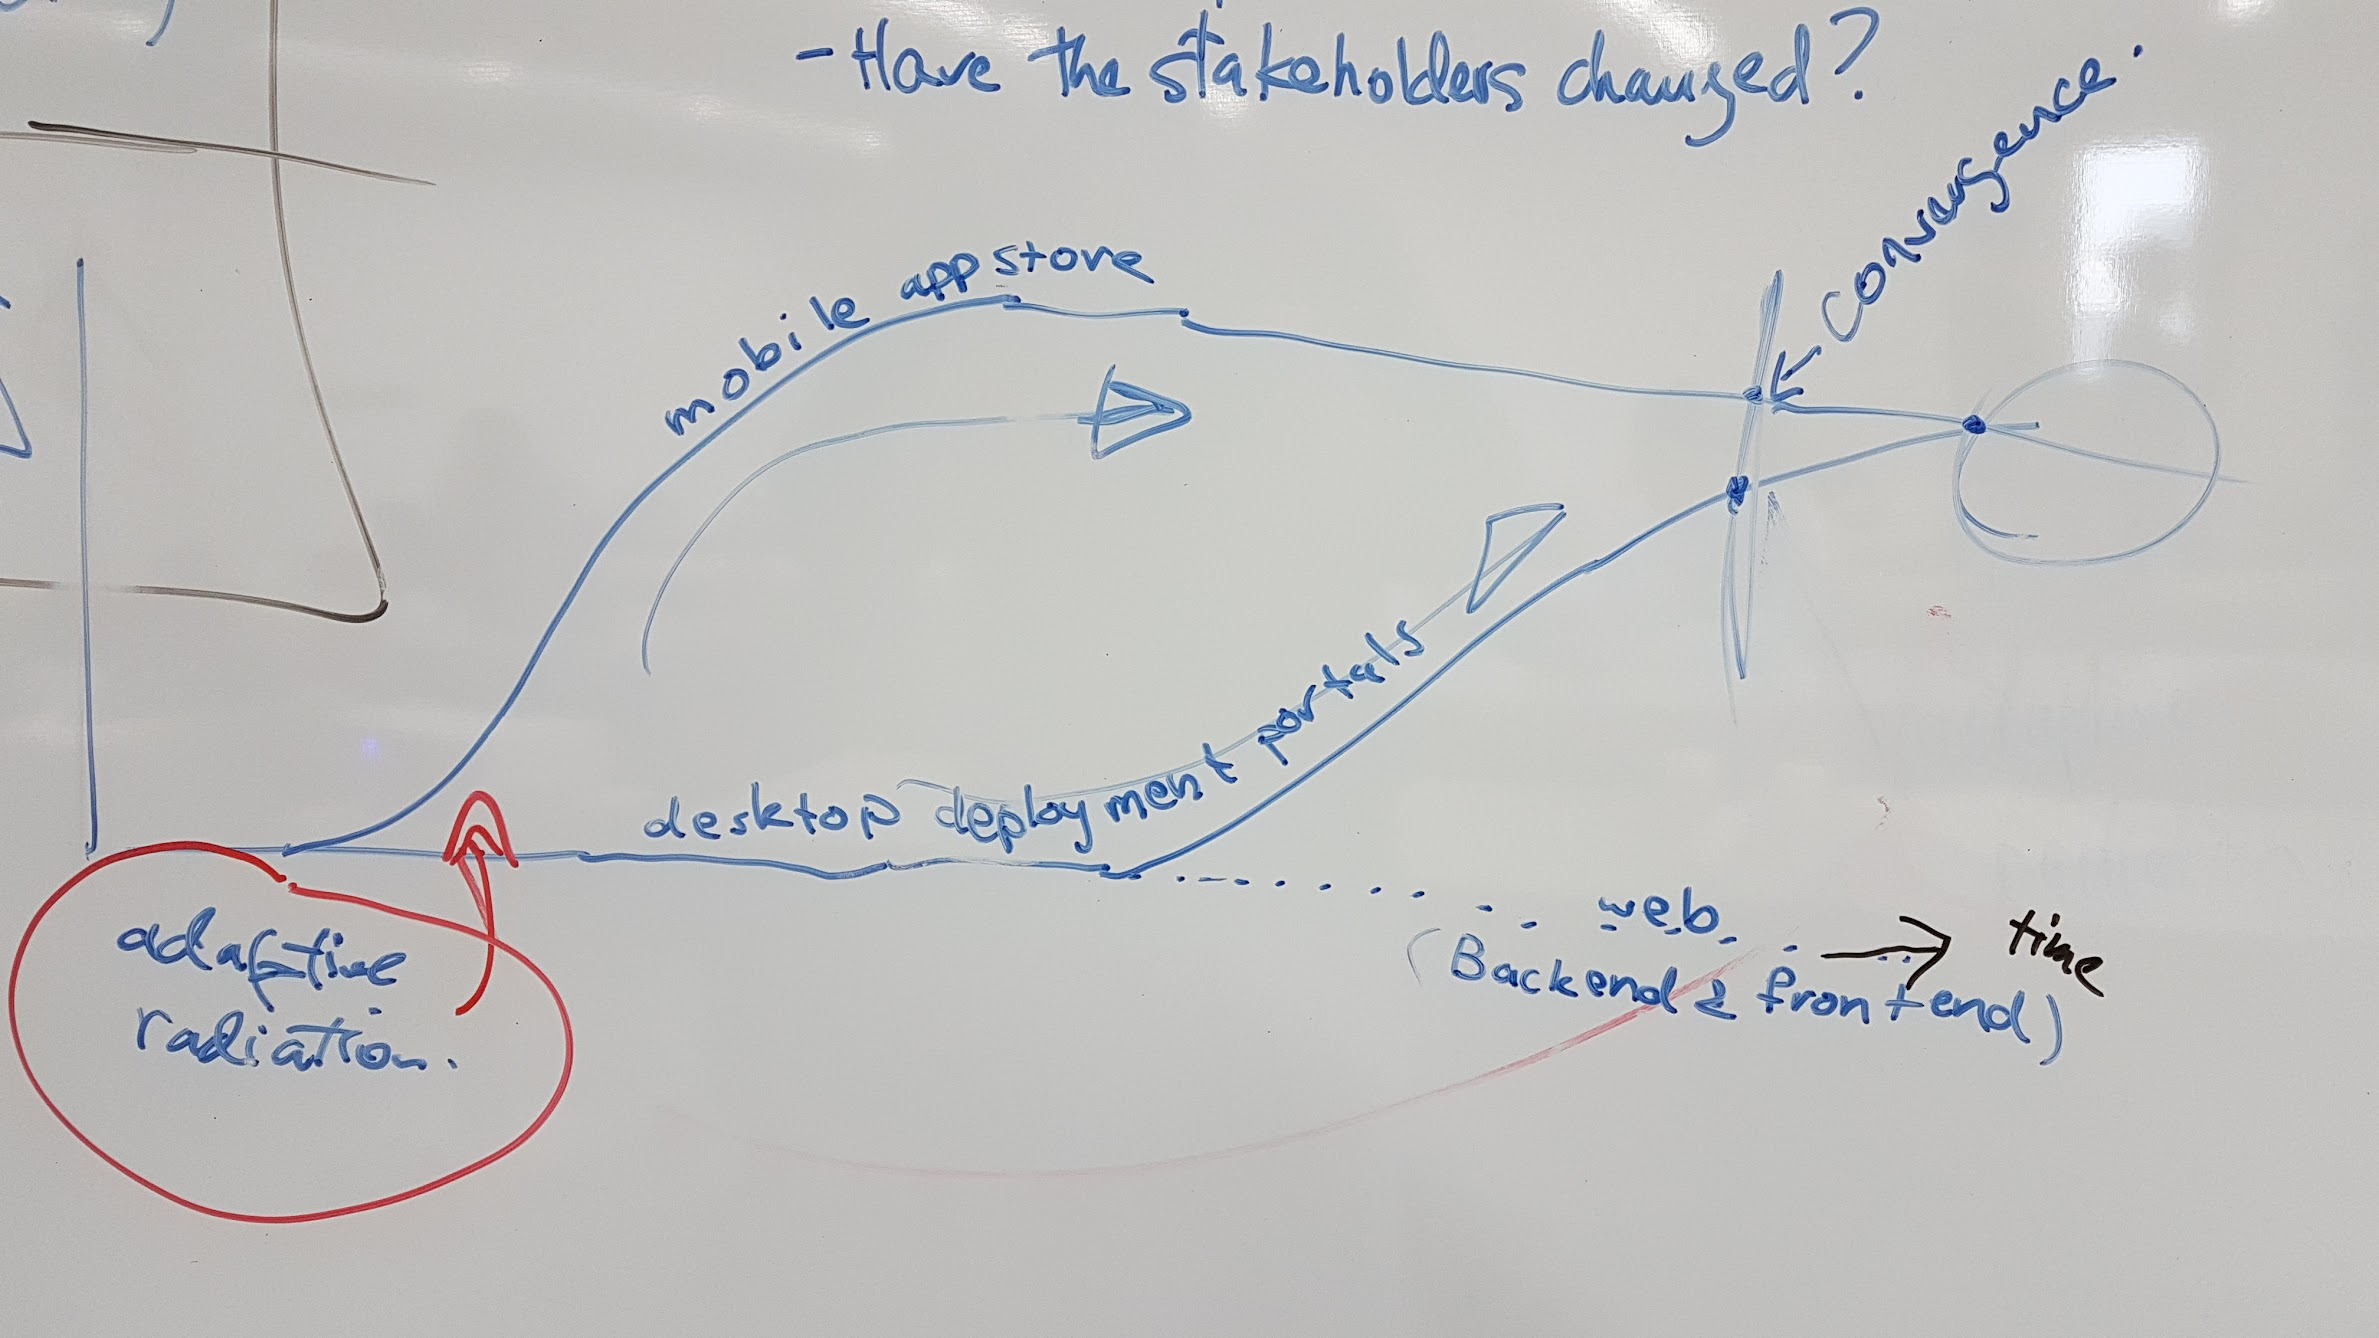
\includegraphics[width=\linewidth]{images/nii-shonan-workshop-152/shonan_hysteresis_diagram_20191210_132528.jpg}
    \caption{Mobile and Desktop Growth and Convergence}
    \label{fig:my_shonan_hysteresis_sketch}
\end{figure}

If the mobile ecosystem is influencing other ecosystems, perhaps this research will also apply to those ecosystems, albeit there are likely to be many distinctions as each ecosystem is distinct and unique.

\newthought{A note on the choice of ecosystem}: 
The practicalities of the research and the case studies where nearly all the work pertains to the Google Android ecosystem also helps in the selection criteria of relevant related works. As the vast majority of active research in the domain of mobile apps also pertains to this ecosystem, this means the topic is richly served in terms of related works.

\newthought{Contents of this chapter}:
The next section provides an overview of the methodology for this chapter, this may be removed pre-submission, nonetheless it is intended to help explain the rationale and the method that underpins the research into related work.

Subsequent sections are organised to provide the context of the research. There are two strands of existing research that this research builds on The first strand comes from software development generally in terms of: development practices, software quality, including measuring software quality, and then the use of software analytics. The second strand is the app store ecosystem and the effects it places on software development and engineering.

These two strands both affect development practices when developing, testing, releasing, and maintaining mobile apps. A particular aspect of developing mobile apps - feedback - is further developed in terms of the feedback that's available to app developers and the research into several of these forms of feedback. The final topic is existing research into crashes and freezes of mobile apps - these are both indicators of poor quality-in-use of the mobile app.

\begin{figure}
    \centering
    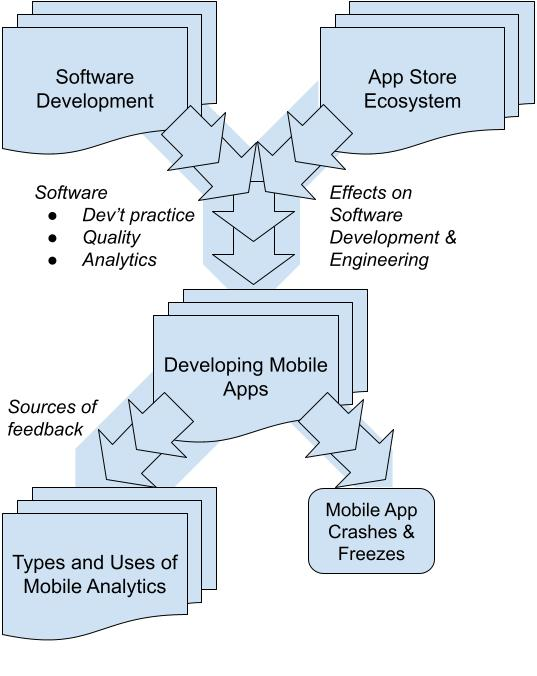
\includegraphics[width=\textwidth]{images/my/related-work-chapter-structure-27-jul-2022b.jpeg}
    \caption{Structure of this related work chapter\\ Source: \href{https://docs.google.com/drawings/d/1DosM__BfTGqoIYkkkltbyDreCT5wYC1Z0mR9i1ZSxWc/edit?usp=sharing}{Google Drawing}, access limited to collaborators to this thesis.}
    \label{fig:related-work-chapter-structure}
\end{figure}

% Reinstate the following once I've completed the first complete draft of the following sections.
% starting with research into app stores and their effects on software development and engineering \ref{rw-app-stores-and-their-effects-on-software-development-and-engineering}...

\section*{Notes on the proposed tactics and topics for the related work chapter}
Marian suggests I aim for writing brief, one-paragraph summaries and apply the T tactic of the broad literature, the top bar of the T are the many and various papers on a topic, and I'm picking these ones that are most directly germane to my research which become the vertical bar of the T.\pending{I'm still currently more verbose than this :(} 

Marian also suggested I might end up with two or a maximum of 3 levels of Ts. The higher level would be on Software Quality Improvement. The lower level would be on mobile analytics.

Where others have done similar work they've done so in other ways eg MSR rather than focusing on the development teams. When I observed the teams the effects of the processes, artefacts, and the tools emerged. This is why I've picked these 3 aspects and 6 perspectives. 

\subsection*{Some notes on the methods used for the literature review}

\begin{figure}
    \centering
    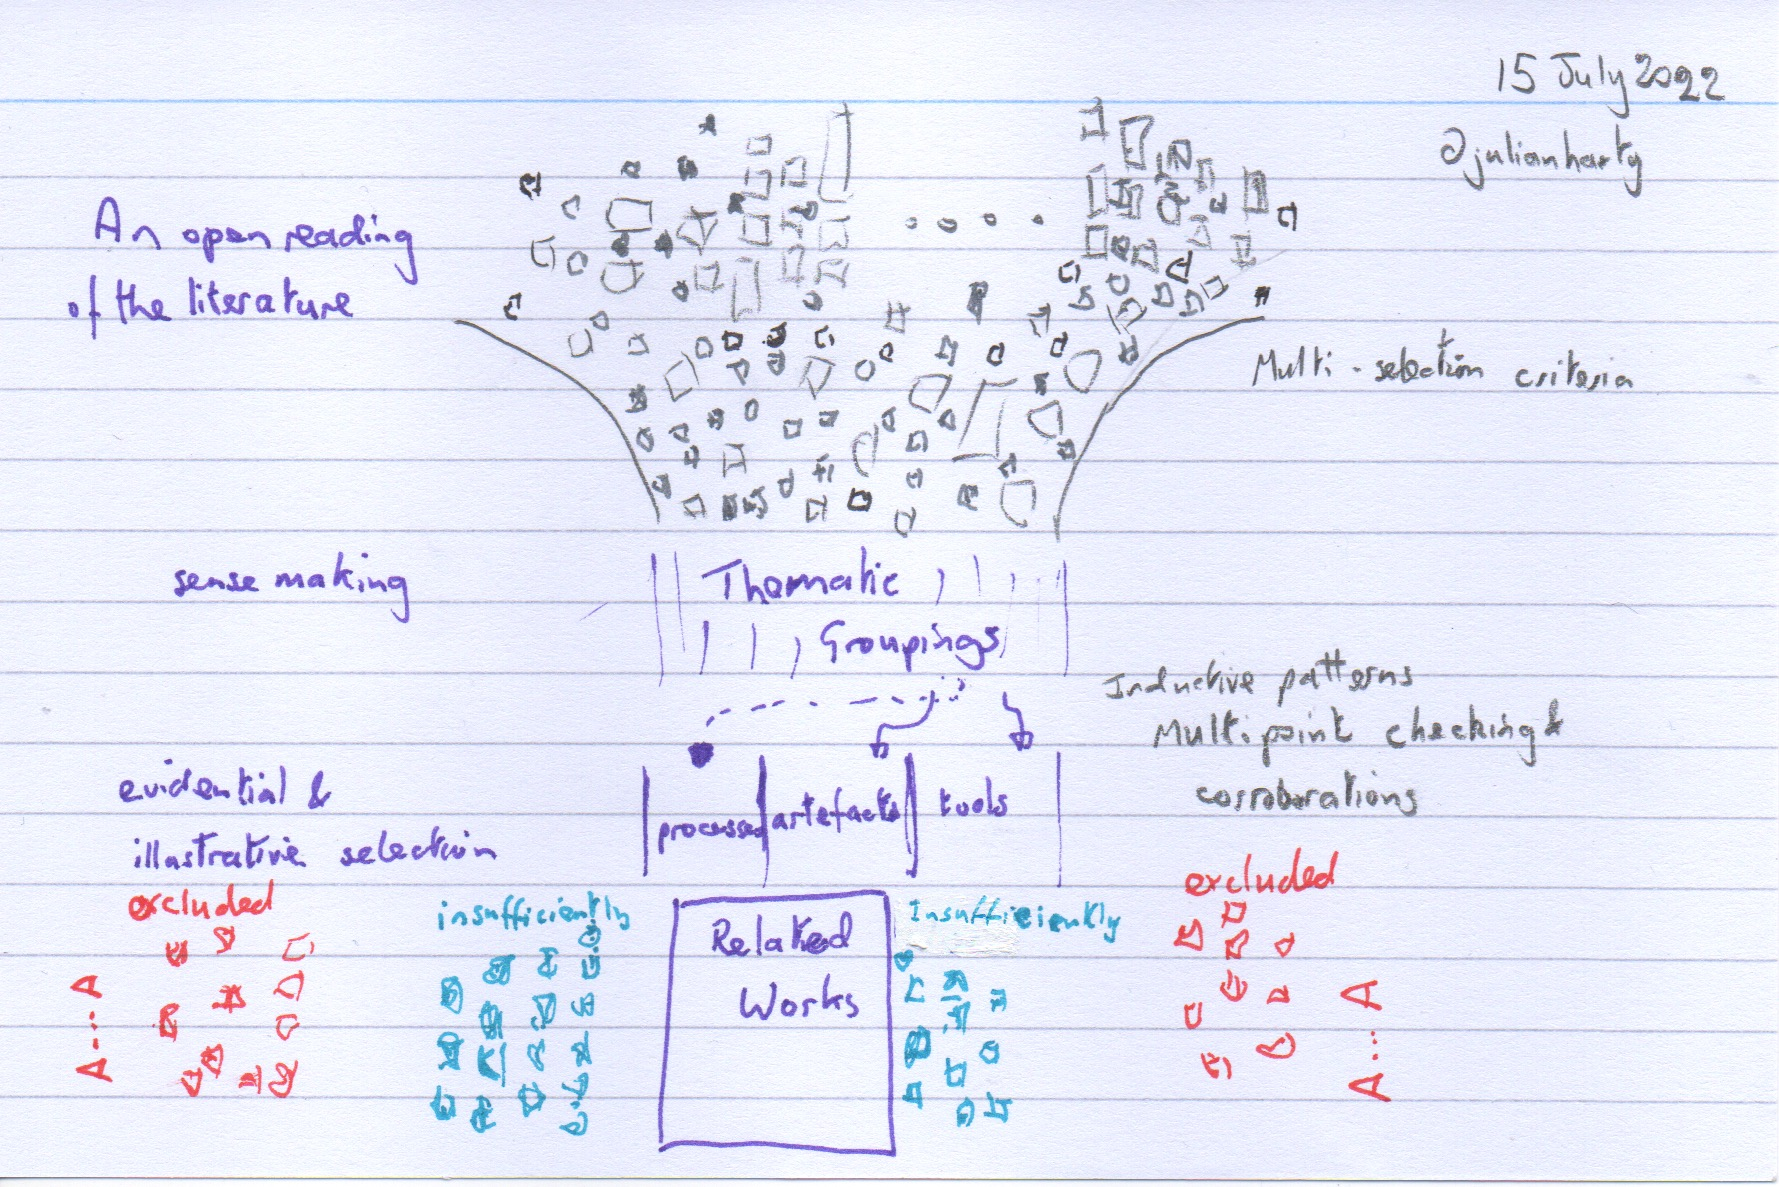
\includegraphics[width=\textwidth]{images/rough-sketches/literature-review-overview.jpeg}
    \caption{Overview of the literature review process and outcomes}
    \label{fig:literature-review-overview}
\end{figure}

Figure \ref{fig:literature-review-overview} illustrates my approach to researching prior work in the use of mobile analytics by app developers in order to measure and improve the stability/reliability of their mobile apps in the field/in the wild. Various searches, including keyword, tags, and related items, were incorporated into the searches. Initial sources included Google Scholar to find the more research oriented materials and Google Search particularly for grey materials, helped provide initial material to seed further searches. Specialist search tools were used where sites provided them, for instance on stack exchange sites such as StackOverflow, GitHub.com, acm.org, ieee.org, and medium.com their respective search engines were used frequently. Where practical copies of material has been preserved privately and backed up using at least one commercial, paid-for, cloud file storage service.

Multi-selection criteria are used to select material that appears of interest, relevant, and plausible. Generally bibliographic entries were obtained and these where checked for accuracy and completeness. Grey material seldom has a bibliographic entry, these were created, generally by hand, and preserved.

Through a process of sense-making, cross-checking, and corroborations various thematic groupings emerged together with potential relationships between the thematic groups. On reflection three clearly distinct and vital aspects emerged in the related work - the development practices used by mobile app developers, the artefacts they create and maintain, and the mobile analytics tools the developers use. These were further refined into six perspectives, using a three-by-two matrix: the x-axis incorporates the three aspects of processes, artefacts, and mobile analytics tools; the y-axis focuses on the current \emph{what is}, and \emph{what might be} in terms of making improvements.\pending{Arosha suggested three pillars which sounds good.}

The research materials and the bibliographic entries are maintained online. The most relevant ones are included in this thesis, many more are maintained in an `outtakes' folder, for example as `fieldstones'~\citep{weinberg2006weinberg} or in an insufficiently-related-works chapter. There's also an `excluded biography' file which helps reduce unnecessary repetition or groundhog day like practices. In the figure (\ref{fig:literature-review-overview}) the two \texttt{A ... A}'s wraps around - excluded works and insufficiently related works are similar distanced to this related works chapter.

In reading the literature various \textit{false friends} emerged, papers that first appear relevant because of their titles and/or abstracts but turn out to be on very different topics. 
Knowing about the concept of false friends and having pragmatic strategies to deal with them is important to avoid misunderstandings or misleading application of their work, 
based on \citep[p. 1833]{chamizodominguez2002_false_friends_their_origins_and_semantics_in_some_languages}. 
\citet{shaw1989_comparing_conceptual_structures__consensus_conflict_correspondence_and_contrast} uses the term 'conflict`, where, \emph{``experts use [the] same terminology for different concepts"}~\citep[p. 3]{shaw1989_comparing_conceptual_structures__consensus_conflict_correspondence_and_contrast} (and, indeed, using their terminology here there is a `correspondence' where experts use two terms to describe the same concept e.g. `false friends' and `conflict' both describe the same concept.). For this research my work was limited to recognising false friends and identifying some examples. 

So somehow I should aim to have the chapter structured with the following topics:\pending{This is a note to myself and needs replacing as I refine the chapter.}
\begin{enumerate}
    \item \textbf{Software Quality [Improvements] for mobile app developers}: Software Quality has been a contested topic for decades with no single accepted coherent agreement on what form(s) it takes, how software quality is measured, etc. Then comes the similarly vexed challenge of determining the concept and application of improvement in the quality/qualities of software. 
    \item \textbf{Mobile Analytics}: Research into \textbf{Processes, artefacts, and tools} necessary when using mobile analytics for improving software quality/qualities. These groupings emerged during the analysis of the literature and through understanding the practices of app developers.
    \begin{itemize}
        \item \textbf{Processes}: a.k.a. Analytics in Use - research into the processes developers use when they use mobile analytics
        \item \textbf{Artefacts}: things the developers create and maintain as part of their development work. Some of these are generated, in particular the app binary that is destined for end users once delivered by the app store.
        \item \textbf{Mobile Analytics Tools}: that the app developers use are worth researching in order to learn about their characteristics.
    \end{itemize}
\end{enumerate}

\subsection*{Software Quality Improvements for mobile app developers}
Here topics might include the measures that have been used by app developers to measure software quality - as confirmed by research literature and grey materials. I suspect this is where I'd include sources of information about software quality (\secref{rw-sources-of-info-on-software-quality-for-devs-of-mobile-apps}).

\subsection*{Development Processes for mobile apps}
Here topics include how the developers are perceived to work when they develop mobile apps, how they spend their time, how they structure and organise their work, etc. I suspect software testing fits here as well as how devs make mobile apps (the artefacts e.g. build scripts would go in the artefacts section).

\subsection*{Artefacts for mobile apps}
There's no end of research on artefacts from various subsets of opensource Android projects. Quite how well these reflect the population of shipping mobile apps (in Google Play in particular) is open to discussion. I can potentially include my joint research on logging practices as we aimed to only analyse projects where the codebase was actively maintained, etc. Research into logging practices by devs might also fit here (however how they use logging would be part of the section on development processes).

\subsection*{Mobile Analytics (and Mobile Analytics tools)}
I think it's germane to include research on the use of mobile analytics and any research into the tools, including the SDKs, data leakage, privacy, etc.

\subsection*{Thoughts on the above organisation of the related works}
As I've written the notes for each of the previous subsections I've had several instances where I've written about a single topic split across processes and artefacts. Perhaps it'd be better to keep the topics together and then summarise the topics by explaining there's a key distinction between the artefacts that exist and how they're used in practice. If so, then the alignment with the six perspectives would occur towards the end of this chapter rather than being used throughout. Let's see.

 % Moved the content to a separate file to reduce noise for the reader of the chapter in latex.


\section{Software Development}
% For the purposes of this research there are at least two camps in research. The first camp is where the research comes from the field and is applied in the field of production, shipping software and the second camp seeks ways to improve the tools, techniques, and results \emph{without} dealing with the practical aspects. The work of the second camp remains unused in reality and oft only reviewed in-passing by other researchers who want to claim their research generates better `results' than that of the other camp members. The second camp's work overall is on an orthogonal path to the work and world of practitioners. The gulf seems wide between these two camps.

%%% Rationale for including this topic 
Mobile apps are developed using similar practices to other modern software projects, however there are key distinctions/differences such as: the build, packaging, and release processes (which are relatively similar to those for software apps generally), how analytics is designed, implemented, and how analytics works all differ. There are also nuances in the effects of software quality as measured by the app store which are important for us to be aware of.

This section, and associated subsections, provide context for the more specific domain of mobile apps, covered in \secref{rw-developing-mobile-apps-section}~\sidenote{As an observation there appears to be little research into desktop apps, such as those available on MacOS. However, research in that area is outside the scope of this research.}.
 
This section covers the following topics: \secref{rw-software-development-practices-topic}, \secref{rw-software-quality-including-measurement-topic}, and \secref{rw-software-analytics-topic}.

\subsection{Software development practices}~\label{rw-software-development-practices-topic}
Jez Humble is a well respected leader in modern software development practices who popularised the concepts of Continuous Delivery and DevOps. In \sidecite{humble2018_continuous_delivery_sounds_great} he argues the benefits of using continuous delivery to reduce risks and transaction costs. to create fast feedback loops, and work in small batches. He also believes it can be applied to any software and any domain. He concludes: \emph{``This, in turn, increases the quality of products, allows developers to react more rapidly to incidents and changing requirements and, in turn, build more stable and higher-quality products and services at lower costs.''}~\sidecite[][p. 39]{humble2018_continuous_delivery_sounds_great}. 

To be successful in applying continuous delivery he identifies the importance of continuous, daily improvement and constant discipline to seek higher performance. Can we assume continuous delivery is suitable for mobile apps and can be applied by developers of those mobile apps? 


\subsection{Software quality, including measuring software quality}~\label{rw-software-quality-including-measurement-topic}

Early work, presented at ICSE in 1997, compared two approaches to software testing - debug testing and operational testing~\sidecite{frankl1997choosing_testing_for_reliability}. Their research considered the two approaches including their efficacy at improving reliability of the software being tested. In their work they challenged the focus on faults which they stated was nebulous and not necessarily the best term to use to describe what happened when failures were detected or when changes were made to 'fix' the code that led to the failures. They introduced the concept or notion of \emph{failure regions}, which could be \emph{``eliminated by a program change''}[p. 70]. Their work and their concepts align well with the use of mobile analytics to identify failures, and failure regions that are detected by mobile analytics and potentially addressed by changes to the program \emph{i.e.} the mobile app. We will revisit this paper in \secref{rw-mobile-app-crashes-topic}.


%Measuring software quality

One of the challenges has been to find ways to measure beyond an app, to behaviours that are externally observable but not easy to measure within an app. Unresponsiveness of software is a particular concern for mobile apps where apps stop responding for longer than deemed acceptable. Google Android coined the term ANR (TODO replace with glossary entry) for when the application stops responding. One of the challenges has been how to detect and measure these, particularly remotely on end-user devices. 

An opensource project provides Android developers with a mechanism to detect and report ANRs in their application. It includes support to report the ANRs to various crash reporters~\cite{salomonbrys_github_anr_watchdog}. (Two of the four listed (Crashlytics and HockeyApp) have been acquired by Google and Microsoft respectively). Note: In 2012, Google was asked to provide a facility to detect ANRs from the application~\footnote{\url{https://issuetracker.google.com/issues/36951741}} so developers would be aware of them and be able to address them. The issue was marked obsolete by Google in 2014 without comment. Approximately six years later, in 2020, Google Android launched an API call that apps can use to determine whether the app was previously quit by the operating system (see \secref{tata-chapter-section-design} for more detail). 

\subsection{Software analytics}~\label{rw-software-analytics-topic}
Software analytics includes the use of analytics to measure and potentially improve processes, products, and software tools. Some of the early published research came from Microsoft Research. For example, Buse and Zimmerman wrote a short paper in 2010 which helped establish the field of:~\emph{``Analytics for Software Development"}~\sidecite{buse_analytics_2010}. The first figure in that paper is reproduced here as~\ref{fig:software_analytics_buse_and_zimmerman_2010}. They had derived that figure from a more general business-focused diagram in Davenport and Harris's book~\emph{``Analytics at work: Smarter decisions, better results"}~\cite{davenport2010analytics_at_work},  in Figure 1.1, titled\emph{``Key questions addressed by analytics"} and found in page 7 of ~\sidecite{davenport2010analytics_at_work}). 

Buse and Zimmermann
\begin{figure}
    \centering
    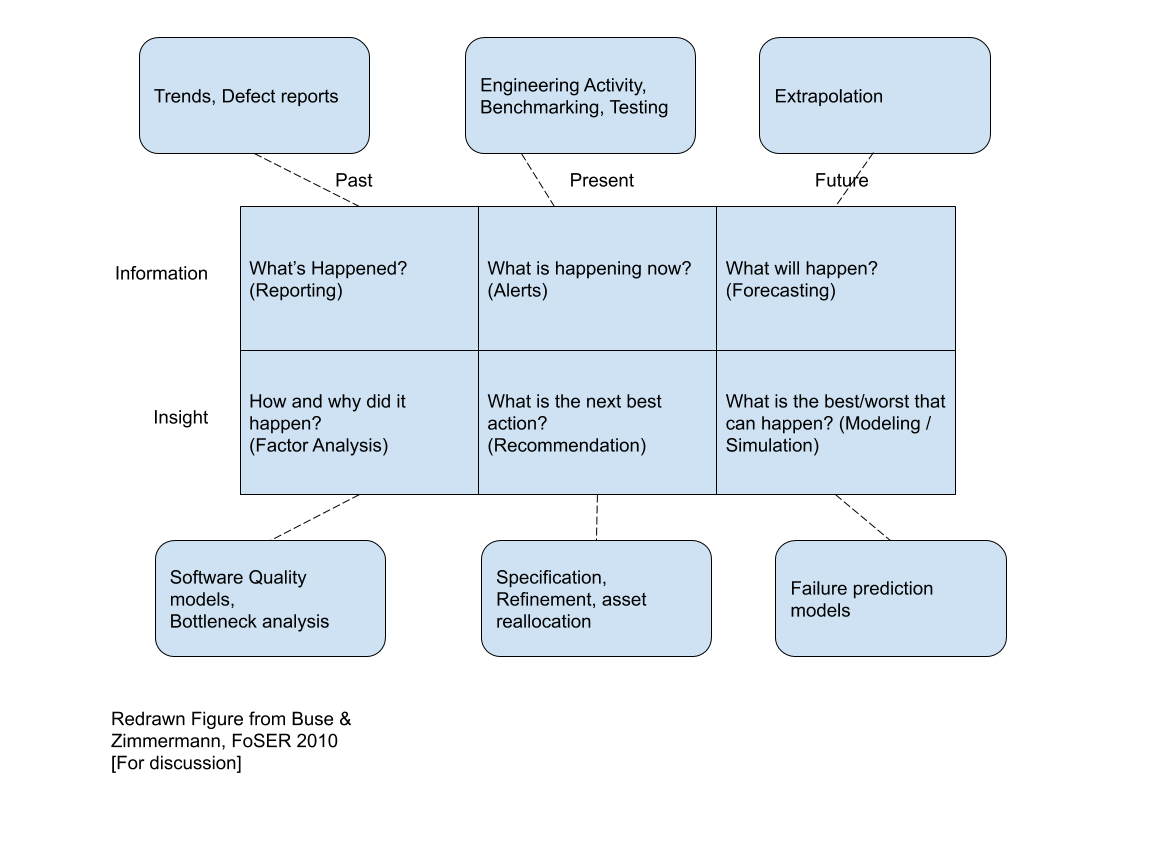
\includegraphics[width=14cm]{images/Buse_and_Zimmermann_2010_figure.png}
    \caption{Software Analytics, Buse and Zimmerman (2010)}
    \label{fig:software_analytics_buse_and_zimmerman_2010}
\end{figure}


In the Buse and Zimmermann paper they \emph{``distinguish between questions of information which can be directly measured, from questions of insight which arise from a careful analytic analysis and provide managers with a basis for action.''}~\cite{buse_analytics_2010}.

\subsubsection{The development managers' perspective}
\emph{``Information needs for software development analytics"}~\cite{buse2012_information_needs_for_software_development_analytics}. They asked 110 Microsofties, a mix of development leads and managers about their use of software development analytics. MUST-DO discuss how my work and their guidelines for software development analytics align. What does my work add to their work? What does it provide that they identified back in 2012? Their focus seems to be more on the code than the product of the code (apps and the services (and the qualities of those services) those apps provide to end users). What information do mobile app developers need in terms of improving the reliability of their apps? How can the developers make good decisions in this area?


\begin{figure}
    \centering
    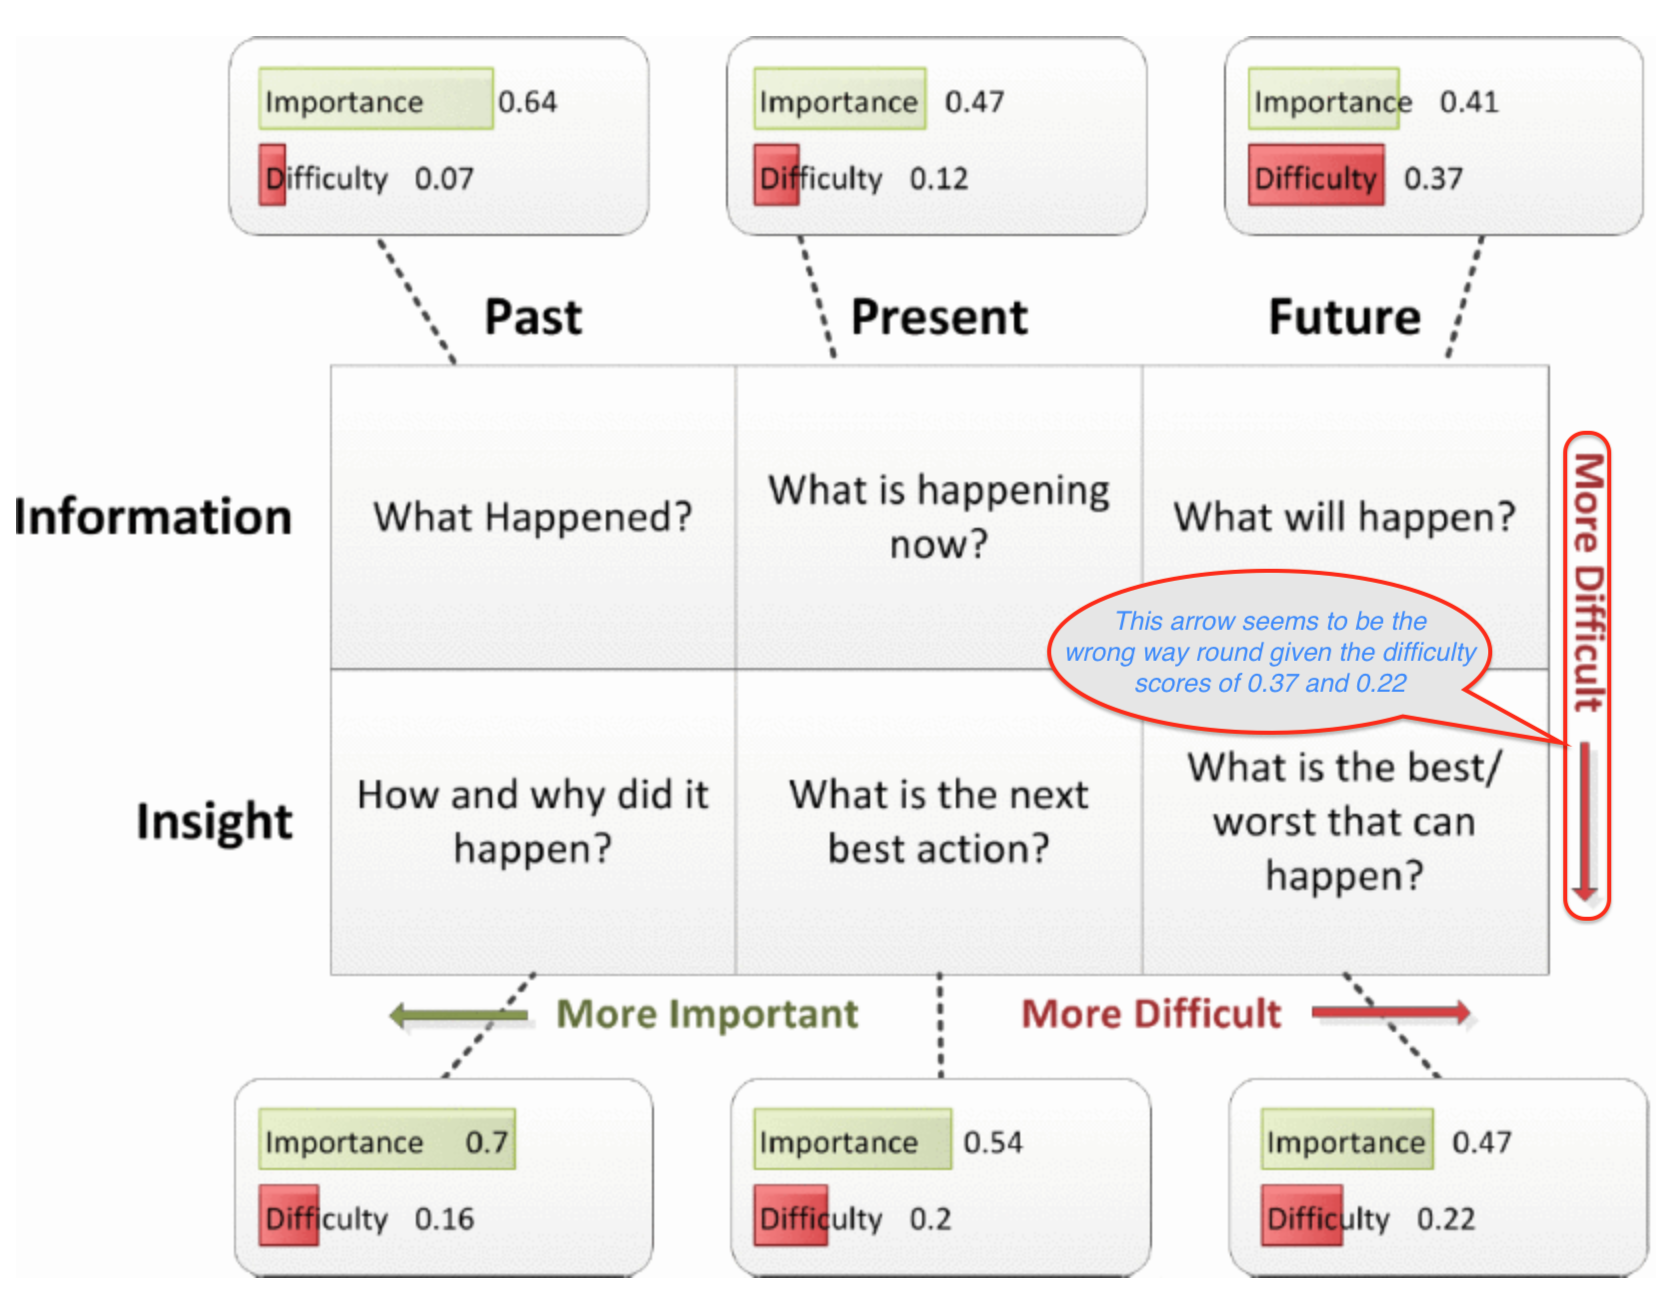
\includegraphics[width=\linewidth]{images/related-work/buse2012-edited-figure-2.png}
    \caption{Revised Figure 2 from TODO}~\footnote{\cite{buse2012_information_needs_for_software_development_analytics}}
    \label{fig:buse2012-edited-figure-2}
\end{figure}


\begin{itemize}
    \item ~\emph{``we ultimately want to} empower software development teams to independently gain and share insight \emph{from their data without relying on a separate entity"}
    \item \emph{``Analytics can help: monitor a project; know what's really working; improve efficiency; manage risk; anticipate changes; evaluate past decisions."}
    
    \item Oddly, Figure 2 in their paper seems to have a mistake in the direction of More Difficult from Information to Insight, see~\ref{fig:buse2012-edited-figure-2}.
    
    \item \emph{``In other words, both developers and managers find it more important to understand the past than try to predict the future; echoing George Santayana, “those who cannot remember the past are condemned to repeat it.”"}.
    
    \item From Figure 4 in their work, Failure Information (\emph{``reports of crashes or other problems"})is in the top 3 that the development leads would use and top for managers when making decisions relevant to their engineering process. Telemetry (\emph{``user benchmarks"} would be used by around 80\% of development leads and 90\% of managers in the survey.
    
    \item \emph{``The landscape of artifacts and indicators in software engineering is well known, but the concrete decisions they might support are not. We conjecture that understanding how managers and developers can make use of information is critical to understanding what information should be delivered to them."}. My research somewhat inverts this by looking at what's being delivered in terms of commercial, pre-existing mobile analytics and considers how that information has been used to improve the reliability of the mobile apps that were the source of the raw information.
    
\end{itemize}~\cite{buse2012_information_needs_for_software_development_analytics}.

\subsubsection{Learning from Windows Error Reporting}~\label{rw-learning-from-wer}
The data collection and analysis of Android Vitals has some similarities with Microsoft's \acrfull{wer}\index{Windows Error Reporting (WER)} which they describe in an article in 2011~\cite{kinshuman2011_debugging_in_the_very_large} and a longer conference paper from 2009~\cite{kinshuman2009_debugging_in_the_very_large}. Similarities include both mechanisms being designed to work effectively at scale of at least a billion end-user machines/devices, capturing crash data, and using error statistics as a tool in debugging. Differences include the platform (Android), the lack of automatic diagnosis (which WER provided), and most relevantly, Google provides several million third-party developers with access to data for the apps they are responsible for and provides them with various comparative analytics of the technical performance of their app compared to those apps of their peers. (Microsoft provided 700 third-party developers, for instance of device drivers, with WER information, and the paper provides a concrete example of how one vendor addressed the top 20 reported issues for their code, and how the fixes percolated out to the end users and halved the percentage of all kernel crashes attributed to that vendor (from 7.6\% to 3.8\%)). Statistics-based debugging, described in these papers, was used in Microsoft's WER and may also apply when developers use mobile analytics.

\subsubsection{Beyond Microsoft}
Microsoft are not unique in publishing research about the use of software analytics. A company, Softeam, used a software analytics platform to collect feedback from their customers and systems with the aim of improving the software quality of their systems~\cite{bagnato2020_challenges_and_benefits_from_using_software_analytics_in_softeam}. They use \url{https://github.com/q-rapids}, a ``Quality-aware rapid software development. H2020 Project (Grant no. 732253)". There are relevant publications listed at \url{https://www.q-rapids.eu/publications}.

\subsubsection{Connecting failures with software analytics}
In a short paper~\sidecite{kidwell2015_toward_fault_taxonomy_application_of_software_analytics}, the authors propose combining fault classification and software analytics for five types of decisions. These are: targetting testing, release planning, judging stability, targeting training, and targeting inspection of software. failure data mined from software analytics tools such as crash reporting tools helps to bring their concepts and ideas to life. Their paper provided initial indicative evidence of their proposals through evaluation of changes to source code for the Eclipse software and discusses the measurement of refactoring to provide more accurate and relevant measurements of the efficacy of the refactoring, rather than considering approaches to improve mobile apps.

\subsubsection{Caveats with software analytics}
% This might be better placed in the discussion or later chapter. TBD.
Using software analytics leads to several \textit{caveats} to consider the `so what' aspects and whether the research is being done well. 
\emph{``Software Analytics, so what?"}~\cite{menzies2013_software_analytics_so_what} to set the context.

\emph{```Bad Smells" in software analytics papers'}~\sidecite{menzies2019_badsmells_in_software_analytics}.

A couple of examples of risks and concerns when using mobile analytics 
\emph{``How Does Misconfiguration of Analytic Services Compromise Mobile Privacy?"} ICSE 2020. This in turn refers to \emph{``Alde: privacy risk analysis of analytics libraries in the android ecosystem."} 2016, and \emph{``Bug Fixes, Improvements, ... and Privacy Leaks - A Longitudinal Study of PII Leaks Across Android App Versions."} 2018.


\section{App Stores and their Effects on Software Development and Engineering}~\label{rw-app-stores-and-their-effects-on-software-development-and-engineering}
% Software developers have flocked to develop mobile apps as that's where billions of users find and use software. In the era of mobile apps before smartphone app stores the device manufacturers and the carriers were the dominant parties. Developers provided their apps directly and/or via carriers and/or a variety of third-party app stores. The ecosystem shortly before the point of inflection is nicely captured in \sidecite{lin2009_os_battle_in_the_ecosystem_of_smartphone_industry}. 

App stores are part of an ecosystem that provides and enforces rules while also constrains various choices while also allowing various freedoms for the participants within the ecosystem. The ecosystem needs to sustain competition~\sidecite[][p. 94]{KAPOOR2021_socio_technical_platform_ecosystems_etc} and revenues. The two largest app stores, Google Play and Apple's App Store, each have their own development platform including an IDE and additional software tools, various SDKs, developer programs, release processes, pricing and revenue rules, and so on. 
%They can effectively severe the connection between developers and their market.
Pivotal effects include: the app approval process (which gates any release of the app to the general user population), rules and restrictions on what the binary contains, the signing process, how the app is packaged/bundled. How app quality is measured and assessed (by the app store, at least - devs have a vested interest in having high quality apps as determined by the app store).

App Stores behave as intermediaries between developers and the users of their software. They make various aspects more transparent including pricing, information about the apps, releases, and ratings \& reviews. There are hundreds of thousands of developers of Android apps according to various sources (320,000 in 2017~\cite{wang2017_exploratory_study_of_the_mobile_app_ecosystem}). 

Many of the developers of the apps are relatively junior, in a detailed survey with 82 respondents~\cite[p. 142 and p.134]{francese2017_mobile_app_development_and_management_results_from_a_quantitative_investigation} Given the youth of the mobile app store concept and the prolific growth of mobile apps from zero to millions in a decade the relative youth of mobile app developers is very plausible and as the paper observes there was a high level of specialization and expertise among the developers surveyed.

In an App Store first the developer then the app store are involved in making a release available to some or all of the user population. There are various competing factors that affect when would be a good time to make a release. Too few and an app may be considered stale or neglected, too many and users may balk at the seemingly endless updates and communications costs. Groups of researchers have investigated various aspects of release engineering, including~\sidecite{adams2016modern} that argues the relevance of modern release engineering and the relevance for researchers, and~\sidecite{nayebi2017version} which concentrates on which version of opensource apps should have been released to the app store. Developers, and their stakeholders, want to make more informed decisions about which releases to make; however there does not appear to have been much research into the testing and quality indicators available to app developers before they make their release public.


This research focuses on the Android ecosystem and the Google Play store - the combination is the preeminent platform in terms of userbase, reach, and platform analytics provided to app developers. Nonetheless, this research also includes research into several additional platforms and app stores, e.g. the Window Phone platform with Microsoft's app store and Huawei's app store for Android, where they contribute to this research. % COULD_DO YY suggests adding a table of the various app stores, I'm holding off doing so as it'd take several hours to compile the supporting information and also I'd then be in a dilemma whether to re-include my material on the Amazon Fire and related app store, etc.


App stores and their ecosystem have affected the lives of billions of end users and millions of software developers. They have become the primary route to market for many app developers and their organisations (exceptions include companies who developed strong businesses elsewhere such as Amazon and Netflix). 
From a research perspective, in 2010, early papers were published on various effects of app stores on academic research e.g. how app stores addressed some of the previous constraints such as reaching more users and facilitating the distribution of the apps and feedback from those users. 

Cramer \emph{et al} discussed aspects of \emph{research in the large} and in particular for my research the importance of ``playing by the rules"~\sidecite{cramer2010_research_in_the_large_app_stores}. This research identified the importance of what happens when developers were deemed not to play by the rules (covered in \secref{rw-power-dynamics-topic}) and this research has been shaped to play by the rules of the app store. % Where practical through responsible disclosure of flaws found in 

Miluzzo \emph{et al} introduced other relevant research aspects, \textit{i.e.}  ongoing concerns such as how to assess correctness when there is no \emph{``ground truth"} - a challenge when evaluating mobile analytics for shipping apps; and a software development model of \textit{``deploy-use-refine"}~\sidecite{miluzzo2010research_in_the_app_store_era}, where app development refines the app based on data gleaned from usage of the app. Their paper even explained how a silly mistake caused their app to crash where the app store then delayed the new release of the app by several weeks. Even in 2010 crashes adversely affected the app store's perception of an app.\todo{TBD where should I mention that our case studies used usage data to refine the app to improve the measured reliability of the apps.} % Their work on CenseMe received an ACM Test of Time award, see https://www.cs.dartmouth.edu/~campbell/page-3/


In more recent research, \textcite{wang2019_understanding_the_evolution_of_mobile_app_ecosystems_a_longitudinal_measurement_of_google_play} provided an helpful longitudinal evaluation of the Google Play ecosystem and raises interesting questions and observations about Google Play; but does not seem to consider flaws, or the effects of flaws, in the app store's data collection, algorithms,\textit{ etc.}

In terms of effects of app stores on software engineering practices there have been several seminal papers written by authors at UCL as part of their App Store Analysis Group~\footnote{http://www0.cs.ucl.ac.uk/staff/F.Sarro/projects/UCLappA/UCLappA.html} while it was active (until roughly 2019). Of these papers, \emph{``App store effects on software engineering practices"}~\sidecite{alsubaihin2019app_store_effects_on_software_engineering} combined interviews with a survey to ask developers of their experiences of developing mobile apps and how those experiences differed with developing other software. There are plenty of other papers that consider the app store from various perspectives but they do not cover software quality or mobile analytics.

Of the ten developers they interviewed a couple were for popular apps (800,000 downloads, 2,000 ratings, 1,000 ratings), the rest were for less popular apps. % 0.1% ratings to downloads for a developer of 1M downloads app: https://www.quora.com/What-is-a-typical-ratio-of-reviews-to-active-users-to-downloads-for-iOS-and-Google-Play-apps
Their research identified automatic in-app crash reporting as the most frequent source of bug reports and the second-most frequently addressed in terms of bug fixes (end-user written bugs were addressed slightly more frequently)~\cite[p. 10]{alsubaihin2019app_store_effects_on_software_engineering}. 

Of particular interest was the discovery that the quality of the [source] code was the least important factor to build a successful app according to the survey results and furthermore the number of downloads were the highest measure of success~\cite[p. 13]{alsubaihin2019app_store_effects_on_software_engineering}\todo{Replace repeated citations with \emph{ibid}?}. Note: Google subsequently (but not necessarily because of this research) have placed a lot of focus on encouraging developers to improve the quality of their Android apps in Google Play. 

Their research is one of several that discusses the gaming of app store ratings, such gaming is unsurprising given the importance placed on these ratings and particularly in having mobile apps with high ratings in the app store. Ratings and reviews are one of the topics of the next section \secref{rw-sources-of-info-on-software-quality-for-devs-of-mobile-apps} given their importance in the mobile app ecosystem.

\emph{Future Trends in Software Engineering Research for Mobile Apps}~\sidecite{nagappan2016_future_trends_in_sw_eng_for_mobile_apps} focuses attention on the software development life-cycle, it does not investigate usage or operational aspects. Figure~\ref{fig:nagappan2016_future_trends_in_sw_eng_for_mobile_apps_figure_1_annotated} is an annotated version of their Fig. 1. [on p. 22](\textit{ibid}) where the annotation shows the key operational and usage areas this work did \emph{not} cover. 


% Note this could do with expanding while retaining the citation (which leads to Float(s) lost quite often) I'd prefer the proper begin{figure) that's currently commented out.
    {\centering
    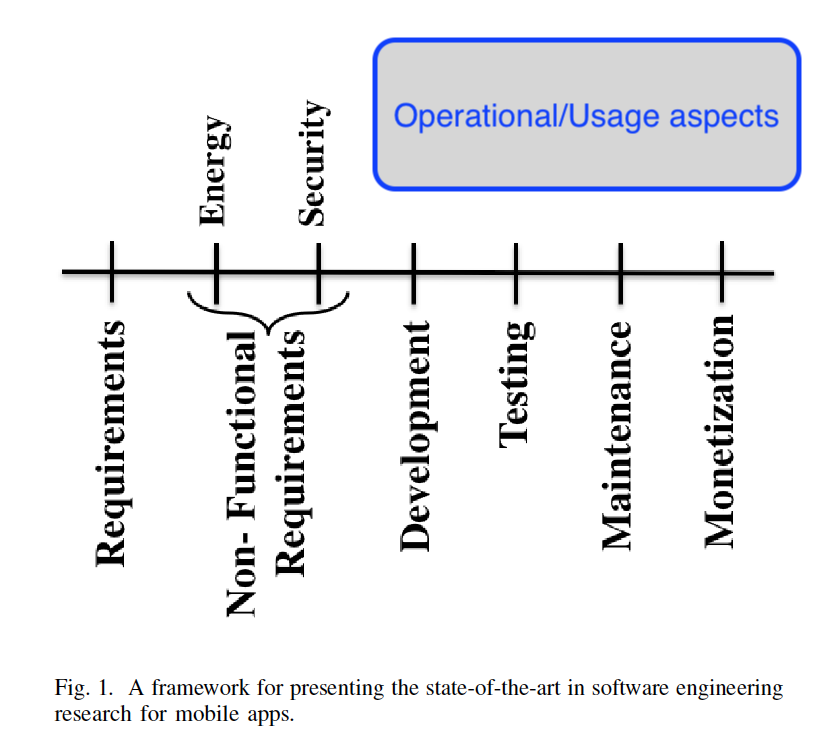
\includegraphics[width=\linewidth]{images/related-work/future-trends-in-sweng-for-mobile-apps-fig-1-annotated.png}
    \captionof{figure}{Annotated version of the framework for presenting the state-of-the-art in software engineering for mobile apps~\cite{nagappan2016_future_trends_in_sw_eng_for_mobile_apps}}
    \label{fig:nagappan2016_future_trends_in_sw_eng_for_mobile_apps_figure_1_annotated}
    } % Thanks to https://tex.stackexchange.com/a/232290/88466

\begin{comment}

\begin{figure}
    \centering
    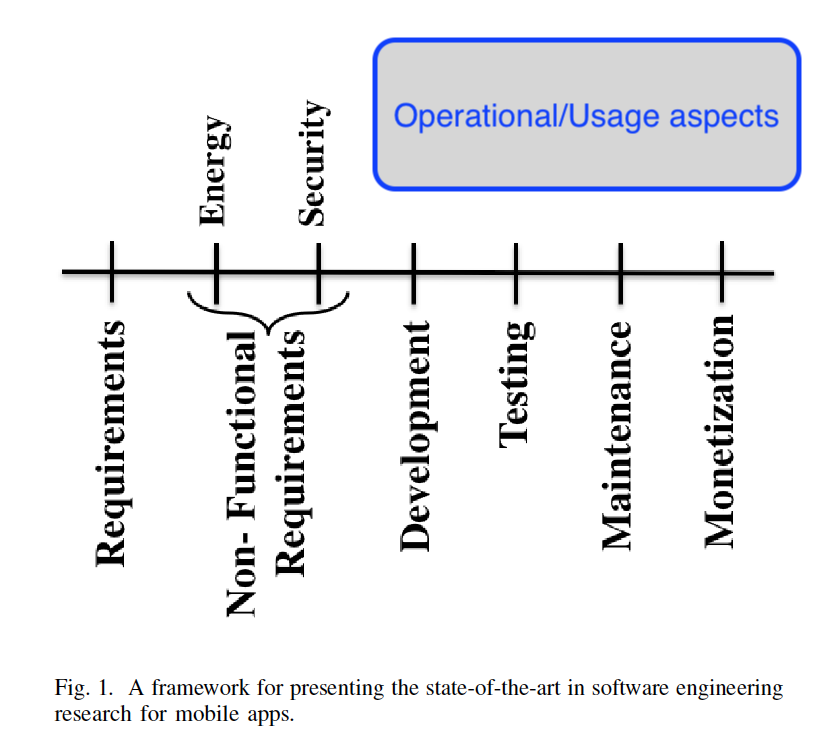
\includegraphics[width=\linewidth]{images/related-work/future-trends-in-sweng-for-mobile-apps-fig-1-annotated.png}
    \caption{Annotated version of the framework for presenting the state-of-the-art in software engineering for mobile apps~\cite{nagappan2016_future_trends_in_sw_eng_for_mobile_apps}}
    \label{fig:nagappan2016_future_trends_in_sw_eng_for_mobile_apps_figure_1_annotated}
\end{figure}
\end{comment}

Mining review data for various forms of data including requests for bug fixes as is using rating as an assessment of goodness. 
Figure~\ref{fig:nagappan2016_future_trends_in_sw_eng_for_mobile_apps_figure_2_annotated} is an annotated version of their Fig. 2 [on p. 23](\textit{ibid}). The annotations include feedback in the forms of ratings and reviews and in the form of mobile analytics. Various sources of information can be used by the development team, of these ratings and reviews are broadly researched, whereas device-level and app-level analytics have not been previously researched.


% Note this could do with expanding while retaining the citation (which leads to Float(s) lost quite often) I'd prefer the proper begin{figure) that's currently commented out.
    {\centering
    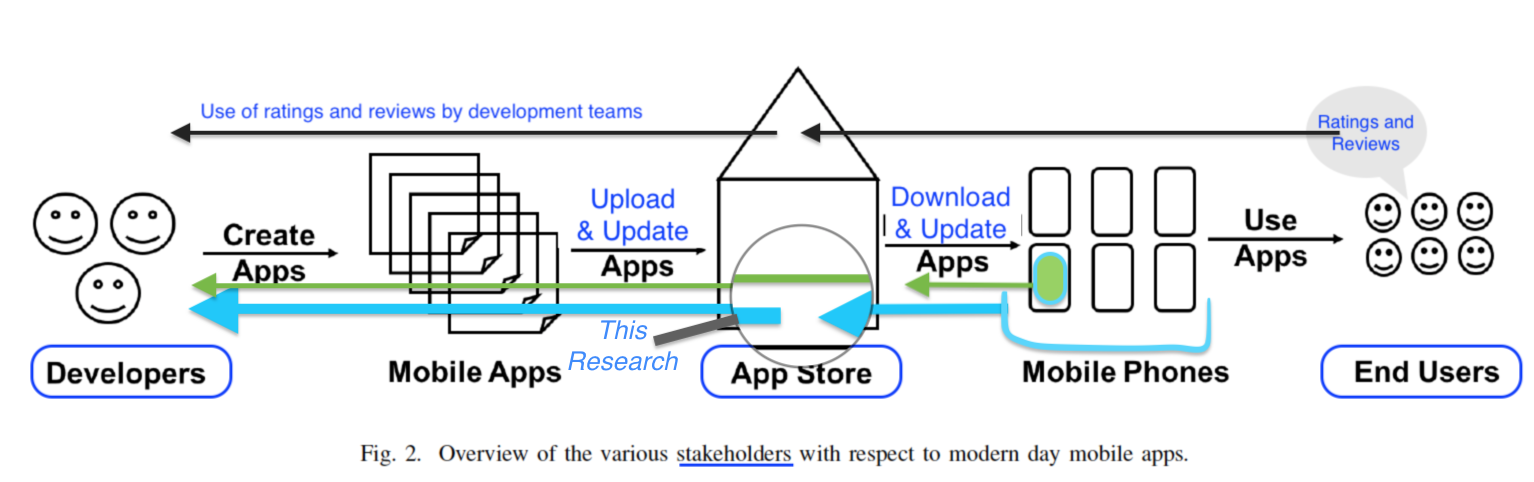
\includegraphics[width=\linewidth]{images/related-work/future-trends-in-sweng-for-mobile-apps-fig-2-annotated-with-highlights.png}
    \captionof{figure}{Annotated version of the various stakeholders in the modern app store ecosystem~\cite{nagappan2016_future_trends_in_sw_eng_for_mobile_apps}}
    \label{fig:nagappan2016_future_trends_in_sw_eng_for_mobile_apps_figure_2_annotated}
    }
  
\begin{comment}
\begin{figure*}
    \centering
    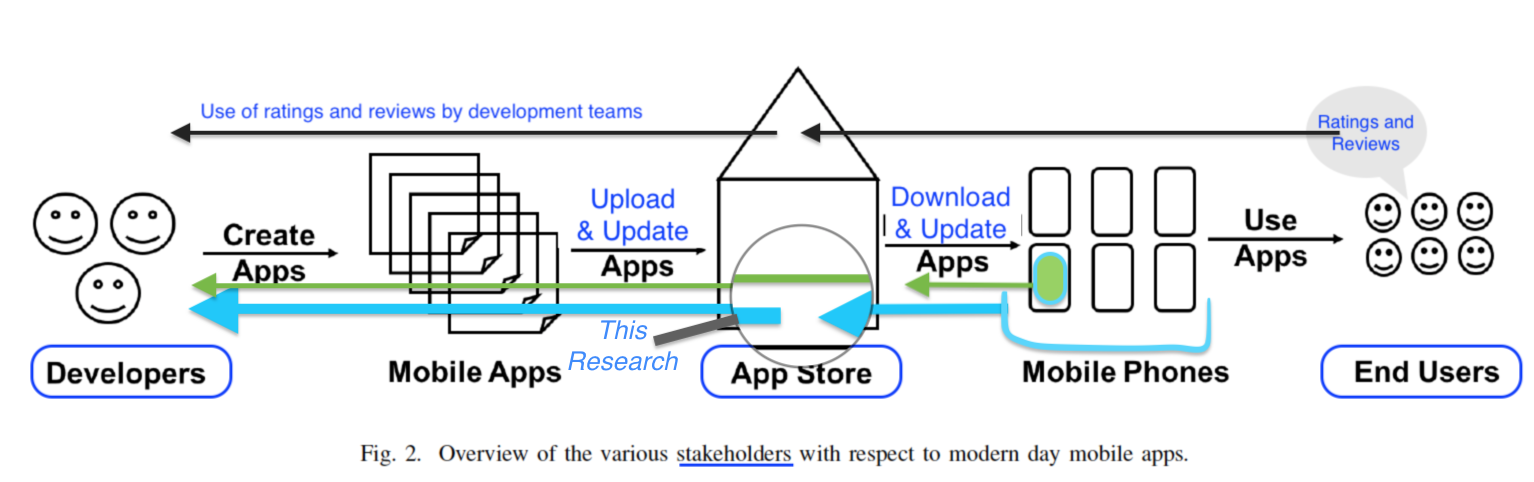
\includegraphics[width=\linewidth]{images/related-work/future-trends-in-sweng-for-mobile-apps-fig-2-annotated-with-highlights.png}
    \caption{Annotated version of the various stakeholders in the modern app store ecosystem~\cite{nagappan2016_future_trends_in_sw_eng_for_mobile_apps}}
    \label{fig:nagappan2016_future_trends_in_sw_eng_for_mobile_apps_figure_2_annotated}
\end{figure*}
\end{comment}  

One of the key challenges identified is restricted access to data held by the app store. The only way they mentioned was to gather historical information by continually mining the app store on a regular basis, [pp 22-23](\textit{ibid}). Perhaps the authors weren't aware that developers of Android apps have access to various historical data about their apps including long term access to all the reviews of their apps. Details of how developers can download these and other reports, including the data structures, are available online~\sidecite{google_play_download_and_export_monthly_reports}.

An area their work did not discuss is whether failure data could, potentially, be a form of requirements? (in a similar fashion to leveraging reviews in the app store to extract `requirements'). And similarly can complaints and failure data be combined to help developers prioritise issues they should consider addressing (the paper restricted the discussion to prioritising issues the developers should be \textit{testing} for).

Finally in terms of this paper, they included two stakeholders, the developers and the end users. The app store (and the people and organisation who provide the app store) are also direct stakeholders in the ecosystem. There are additional indirect stakeholders including advertisers, researchers, and probably many others. 

\subsection{Utility and Service Providers}~\label{rw-utility-and-service-providers-topic}
Developers use software and related services from various providers where the providers are the primary source of any updates. The providers may charge for their offerings and similarly they may mandate various behaviours from developers and their organisations who use the utilities and/or services.

In the context of this research mobile analytics are provided as utilities and/or services by third-parties to app developers therefore it is useful to learn of pertinent research into the use of these utilities and services. Utilities include software tools, libraries, frameworks, and so on; and services may be provided either for some of these utilities or for additional capabilities, support, and so on. Some of the offerings are specific to mobile apps, however many include other platforms such as web sites and/or web apps. Of these examples, an understanding of the use of software libraries helps identify the proclivity of developers to use them and similarly services that apps use are particularly relevant.


\newthought{Libraries: }
Developers can choose to use external libraries to generate revenue (ads)~\sidecite[][p. 407]{li2016_an_investigation_into_the_use_of_common_libraries_in_android_apps}, to \emph{ease the management of HTTP requests}~\sidecite[][p. 73]{belkhir2019_an_observational_study_on_the_state_of_rest_api_uses_in_android_apps} and in their related work they found 98\% of android apps used third-party libraries in their apps~\sidecite[][p. 218]{abdellatif2020_a_multi_dimensional_study_on_the_state_of_practice_of_rest_apis_usage_in_android_app} and on average 41\% of android apps is contributed by common libraries~\sidecite[][p. 409]{li2016_an_investigation_into_the_use_of_common_libraries_in_android_apps}. Using the data in Fig. 5 of this paper (on p. 409) 5\% of the apps included Google Analytics and 2.6\% used Flurry analytics. Note: Industry data indicates mobile analytics are now incorporated in the vast majority of Android apps.  

\newthought{Services: }
Two of the extremely popular categories of third-party libraries are advertising (ads) and mobile analytics.\todo{add examples from research using appbrain examples as a grey data backup/alternative.}
In some ways app developers appear to be similar to their end-users - neither wants to pay up front for what they use.\todo{Add research into the ratio of free to paid apps.} Typically service providers have at least one form of unpaid service offering either time or volume based, many then also have at least one paid-for service offering that do not have the same restrictions of their unpaid offering.

Remote device farms are good examples of services that at least some developers (and/or their organisations) pay for. A relatively dated paper about the then current device farm services provides a useful overview~\sidecite[][]{starov2015_taas_for_mobile_apps_survey} but does not discuss pricing and it predates the now popular service offerings by Google, Amazon, and others. I'm not aware of much research into the use of these device farms apart from some in Brazil IIRC who used an opensource backed test lab service. 

\subsection{Using app store crash analytics to automatically find robustness and reliability failures}~\label{rw-windows-phone-store-crash-analysis-section}
There was a breakthrough stream of work and research that was developed for Microsoft's now defunct mobile app store for Windows Phone devices. That work included mining 25 million crashes~\footnote{Note: The 25 million crashes were a small subset of the total crashes on end-user devices were a subset of the total based on their third footnote ``The developer has no control over the probability.''~\cite[p. 191]{ravindrath2014_automatic_and_scalable_fault_detection_for_mobile_apps}.} that occurred in 2012 on end-user devices when using various apps on their Windows Phones~\cite[p. 190]{ravindrath2014_automatic_and_scalable_fault_detection_for_mobile_apps}. They determined the top 10\% of error buckets covered more than 90\% of crashes~\cite[p. 192]{ravindrath2014_automatic_and_scalable_fault_detection_for_mobile_apps} and discovered a significant proportion of these stemmed from root causes they could generate externally. For example, they could configure a network proxy to return a HTTP 404 response to a network request for network calls made by any of the mobile apps [p. 192].

They built a service called VanarSena to run in the cloud on lots of Windows Phone emulators with the purpose of automatically testing Windows Phone apps. The service automatically instrumented these apps, for instance to add a global Exception handler (the complete set of five injected modules are described in pp. 193..194). The app is exercised using autonomous automated testing tools called~\textit{monkeys} and the service includes a range of fault inducing modules (FIM) [p. 196] that provide inputs and conditions including those that have caused existing apps to crash. 

This paper includes lots of additional practical information that would be pertinent for providers of similar services \emph{e.g.} for other automated testing providers and/or app store providers which we can skip here as they are not closely related to using mobile analytics. Instead, let's concentrate on key characteristics of their work:

\begin{itemize}
    \item Their work built on earlier work of some of the authors where that work was performed at a smaller scale on Android~\cite{ravindrath2012_appinsight_mobile_app_performance_in_the_wild}. They share a common instrumentation framework implemented first for Android then for Windows Phone.
    \item The authors proposed VanarSena could be provided by an app store to help test new releases before they were released in production. The automatic testing helps establish whether the apps handle non-ideal conditions without crashing.
    They describe crash buckets and a) identified commonalities in those crash buckets, b) found a significant subset could be triggered through manipulating inputs, conditions, and responses to the app.
    \item The results of their research included finding 1108/3000 production Windows Phone apps had failures that were detected by VanarSena. They uncovered 2969 distinct bugs in these apps including 1227 that were not previously reported~\cite[p. 202]{ravindrath2014_automatic_and_scalable_fault_detection_for_mobile_apps}. Some of the failing apps had been developed by professionals others by amateurs - this indicates developers often write code that does not cope adequately with non-ideal circumstances.  
\end{itemize}

Several of the authors of the previous paper collaborated with other colleagues at Microsoft Research to extend the work. In ~\textcite{chandra2015_how_to_smash_the_next_billion_mobile_app_bugs} they describe various improvements to their Caiipa service that delivered eleven-fold more crashes and eight-fold more performance problems~\cite[pp. 37-38]{chandra2015_how_to_smash_the_next_billion_mobile_app_bugs}. The core of their paper presents their plans for a sophisticated automated testing system for testing Windows Phone apps together with their goals and challenges. The most pertinent goal in terms of this research would be actionable reports~\cite[p. 36]{chandra2015_how_to_smash_the_next_billion_mobile_app_bugs} together with their use of context data and historical data. 

Given the nature of Microsoft's objectives they did not consider Mobile Analytics or crash reporting SDKs (which include breadcrumbs and the ability to report caught errors, \emph{etc.}). Nor do their papers mention how the app developer's perceived their various tools and services. It's unclear whether they actually involved app developers in their work. Also, given the demise of the Windows Phone platform and app store it appears much of this work has disappeared without a trace.


\subsection{Power dynamics}~\label{rw-power-dynamics-topic}
Grey literature is the main source of the imbalance in power between app developers and the app store, at least in terms of Google Play and Android apps in that store. I have selected four illustrative articles, by four different developers, of the 20+ related articles published on \href{https://medium.com/}{Medium} % More material is available on corporations on mining data from the public  from and via https://jilliancyork.com/
about how they lost access to their apps and in some cases their account. 

In \textcite{martinez2019_google_just_terminated_our_startup_google_play_publisher_account_on_xmas_day} the termination of a personal Google Play account for an indirectly associated developer, via one of the employees of the small company, was attributed to the termination of that company's Google Play account. This story has ongoing updates that lists various developers who have had similar experiences. A similar experience was reported by \textcite{dodson2019_google_completely_terminated_our_new_business_etc} where apparently someone's associated account was the cause of Dodson's account being terminated. As Méa dry noted \emph{``google@play-store: sudo rm -rf org.mtransit.android*''} which happened abruptly within a few hours of sending an email notification to the developer. The reason given in the automated emails was the app was in violation of the ``Deceptive Behavior policy''~\sidecite{mea2019_google_just_deleted_my_nearly_10_year_old_app_etc}. 

In these three instances the developer accounts were reinstated. In \textcite{marcher2021_how_google_terminated-a-developer} the account was not reinstanted and two of his clients also had their accounts terminated. As Marcher notes \emph{``I develop software not just for fun but also primarily for a living. This action not only deprives me of a substantial part of income, but it also forbids me for life to continue my work which is also my passion''}. % See also https://medium.com/@appsrentables1/google-cancels-our-google-play-publisher-account-and-ends-my-familys-source-of-income-97d4e85cd046 and various others (20+ stories)

\subsection{Developers and their app counts}
Before we leave the topic of App Store ecosystems and in particular a developer focused perspective on the ecosystem, the work of \textcite{wang2017_exploratory_study_of_the_mobile_app_ecosystem} looks potentially interesting as it states it looked at the Google Play store from a developer's perspective; the title appears misleading as they actually researched mappings between developers and the number of apps they had in Google Play Store. In other words, the paper concentrates on the characteristics of developers who have many apps in the app store rather than on the software development/engineering aspects.

They estimated there were 320,000 developers, over half of the developers only released a single app. The paper main focus though is on the \emph{``the group of aggressive developers who have released more than 50 apps, trying to understand how and why they create so many apps''}. In terms of this research this paper provides some context on who writes the mobile apps in Google Play, provides an estimate of the population of developers (in 2017).


\section{Developing Mobile Apps}~\label{rw-developing-mobile-apps-section}
Research into the development practices and mechanisms for mobile apps establishes various norms, characteristics, and habits, of app developers. Their work, collectively, is used by billions of people throughout the world. In terms of this research, understanding the development practices and mechanisms is vital. Developers also have a voice and hundreds have been interviewed to learn what's important to them, for example in \sidecite{joorabchi2013_real_challenges_in_mobile_app_development}. They also communicate through various artefacts they create and maintain, again these artefacts have been studied to learn about their work, for example in \sidecite{pascarella2018_self_reported_activities_of_android_developers}.

% Some of the effects of their work in terms of software quality will be covered later in this chapter in \secref{rw-mobile-app-crashes-topic}.

Mobile apps need to be made and developers make them. There are various working practices, apps are made by visionaries, employees, amateurs, and communities. There are various activities involved including development, testing, release, and deployment. % Figure~\ref{fig:my_mobile-app-makers} highlights these activities as part of the overall ecosystem.

% Many mobile app development teams would describe their development practices as Agile or based on along the principles of Agile development. % Solo app developers are less likely to use these practices, nonetheless there has been various research into adaptions of Agile and Scrum in attempts to suit them. Various examples are in the excluded-bibliography.
% Many of these people claim to be ``Agile" in their working practices.

5,000 commit messages (of over 1.8 million identified) were studied that were selected from 8,280 active opensource Android apps where the source code repositories were on github.com. The top three activities were 1) app enhancement, followed by 2) bug fixes, and then 3) project management~\sidecite[][p. 144]{pascarella2018_self_reported_activities_of_android_developers}. 35 of the commit messages were attributed to addressing crashes in the app [Figure 3, on p. 151]. They did not investigate how developers had discovered issues nor whether mobile analytics were affected in the commits, leaving these aspects unknown and unreported.

Relatively early research, published in 2013, identified several key topics of concern for app developers including: a strong need for monitoring and analysis support, for instance to monitor the health of an app. Similarly a major problem was crashes \emph{``which are often intermittent, non-deterministic, and irrecoverable.''}~\sidecite[][p. 21]{joorabchi2013_real_challenges_in_mobile_app_development}. Interestingly, one of the discussion topics was to research testing \acrshort{api}s from App Stores[pp. 22-23] which predates Google Play's Pre-launch reports covered in \secref{tata-pre-launch-reports-topic}.


As mentioned previously, in \secref{rw-utility-and-service-providers-topic}, Android apps incorporate software libraries extensively~\sidecite{li2016_an_investigation_into_the_use_of_common_libraries_in_android_apps}. The extensive use of software libraries, generally provided by third-parties, indicate the developers place significant trust with these third-party developers. Also, their apps contain large volumes of code that is \emph{unlikely} to have been tested by the app developers apart from some sanity and/or smoke testing. Flaws and instabilities in these libraries may be latent until the app is being used at scale by end users. How will the developers learn about the effects of emergent flaws and instabilities?

Note: in terms of trying to understand real-world practices please avoid \textcite{santos2016_investigating_the_adoption_of_agile_practices_by_20_undergrad_students_in_mobile_app_devt} which sounds relevant but only surveyed 20 undergraduate students who took an iOS development course. 

\subsection{Testing Mobile Apps}~\label{rw-testing-mobile-apps-topic}

There has been a tremendous amount of research into practices and tools that might perform better than the mainstream test automation tools available to app developers.

A useful categorisation of testing for mobile apps may be: 
explicitly designed scripted tests, 
automatic robots that navigate and sometimes interrogate target apps, and 
hands-on testing which often vary depending on who performs them and each instance of the testing. 
Where the testing may be performed:
on local physical devices,
on remote physical devices in the `cloud'
on local emulators and/or local simulators, and
on remote emulators and/or simulators.


There has been a lot of research into various artefacts pertaining to mobile apps. Some of the artefacts are mainly generated by end users, for instance ratings and reviews, and others are mainly generated by software developers such as source code. A hybrid artefact are bug reports. These also known as issues particularly for projects based on github.com as it uses that term and developers create bug reports as issues on github.com. Bug reports are a hybrid artefact as potentially anyone can create them including users of the code and the development team. 

That said, for the projects studied in this research they mainly used `issues' and these were mainly created by the project's extended development team (an extended development team may include people involved in project management and/or testing).

\subsubsection{Papers to consider}
\begin{itemize}
    \item Discuss the TestDroid paper! it describes testing that was actually done by developers!~\cite{kaasila2012_testdroid_etc}.
    
    \item \emph{``Is Mutation Analysis Effective at Testing Android Apps?"}~\cite{deng2017_is_mutation_analysis_effective_at_testing_android_apps}.
    
    \item \emph{``Mining Android Crash Fixes in the Absence of Issue- and Change-Tracking Systems"}~\cite{kong2019_mining_android_crash_fixes}.
    
    \item \emph{``How do Developers Test Android Applications?"}~\cite{linares2017_how_do_developers_test_android_apps}. Quote:~\emph{``“I mostly do manual testing due to the limited size of my apps. I sometimes use a custom replay system (built into the app) to duplicate bugs after I come across them. This method is usually combined with manual testing (printing debug information to the log) to pinpoint the cause”."}
    
    \item \emph{``First Steps in Retrofitting a Versatile Software Testing Infrastructure to Android"}~\cite{oliver2018_first_steps_in_retrofitting_a_versatile_sw_testing_architecture}.
    
    \item \emph{``A Large-Scale Study of Application Incompatibilities in Android"}~\cite{cai2019_large_scale_study_of_android_incompatibilities} An oddly insipid paper which promised some interesting run-time issues discovered in their research where the Android version would be a likely cause. However the reproduction package lacked the test scripts or means to reproduce their testing or bug detection. Also, their research now seems to be less relevant in 2020 as Android apparently improved the backwards compatibility \emph{``Yet newer versions (since API 24) had no run-time compatibility issues with apps created in the studied span."}. Their work may well have merit for the research community, It does not appear to have much relevance to developers of real-world Android apps today.
    

    \item \emph{``Intent Fuzzer: Crafting Intents of Death"}~\cite{10.1145/2632168.2632169} TODO Link this to the industrial case study and the Kotlin NPE crash.
    
    \item \emph{``Linares-Vasquez et al. [56] propose MonkeyLab, which mines recorded executions to guide the testing of Android mobile apps."} Their approach records GUI events (click events). Members of the project team (developers, testers, etc.) perform the actions, the authors claim their log collection process could scale to collecting logs from ordinary users. Key limitations include events that aren't purely dependent on the user's GUI inputs, there would also be challenges getting users to accept such an approach where the app records every input they made. Also, they generate GUI events that have x,y coordinates - absolute positioning that may have limited portability to other devices, screen rotations, and so on. Their playback also appears to require rooted devices. There are numerous other limitations described in their paper, nonetheless their work shows promise in terms of detecting and generating patterns the students did not find. It would be interesting to compare the results using accomplished software testers with experience and expertise testing similar Android apps.
    
    \item \emph{``An Empirical Study of Android Test Generation Tools in Industrial Cases''}~\cite{wang2018_an_empirical_study_of_android_test_generation_tools_in_industrial_cases} 
\end{itemize}

There has been a tremendous and sustained research interest in software testing, for instance testing is one of the most popular topics at the ICSE series of conferences~\footnote{\url{https://dl.acm.org/conference/icse}} and the focus of entire conferences including AST~\footnote{\url{https://conf.researchr.org/home/icse-2020/ast-2020}}, ICST~\footnote{\url{https://conf.researchr.org/series/icst}}, and so on. Similarly the application of software testing to mobile apps is a rich topic with sustained interest in the challenges and facets of testing mobile apps.

The facets include automated testing and automated bug reproduction, maximising the `bang for the buck' for instance in selecting which device models would be most valuable to use with finite testing. Understandably given the field where many of the authors work - in research - the vast majority of the research is on software apps they have access to, software their can obtain the source code for (particularly opensource), software they can write, and the people they have available to them (other researchers, students, voluntary participants, and people paid to paid to perform specific tasks). Minute amounts of the work is based on mature, popular software with semi- or fully- professional developers and development teams. Some research projects, particularly CRASHSCOPE~\cite{moran2016_automatically_drr_android_app_crashes}, offer the potential to reproduce some of the crashes reported by Mobile Analytics if the tools are sufficiently available and current to actually use.




\subsubsection{Prioritising devices to test on}

Selection criteria include:
\begin{itemize}
    \item the relative popularity of a single app across the user base for the app, provided by OpenSignal, and reported over a three year period,
    \item the usage of similar, popular, Android apps for two app categories: grouped by device model as measured by a very popular app management app in China,
    \item the devices used most frequently by users who write reviews for the same Android app,
\end{itemize}

One of the research papers close to the area of my research uses usage data for two popular app categories (games and media) gathered through a popular Android management app in China~\cite{lu2016_PRADA}. Their work uses an operational profile to prioritise the device models to select to test both new or existing apps. The management app, called Wandoujia~\footnote{\url{https://www.wandoujia.com/}}, is used by \emph{`500 million people to find apps they want`}~\footnote{According to Chrome Browser's automatic translation from Chinese.}. Daily usage of the top 100 apps in the two app categories was collected for various device models. In various ways the Wandoujia app management app provides similar capabilities to Google Play, including tracking when apps are installed, and in use. The recommendations are coarse-grained. The research measured the accuracy of their predictions for recommended devices with the actual devices that the app ended up being used on once the app had been launched. 

Their work demonstrates that usage data for several app categories was useful to guide developers on the most popular actual device models for their app. They acknowledge several limitations in their work, including their use of incomplete measures such as foreground network activity for usage which don't suit apps that either perform network processing in the background or don't use the network. Other app management services, particularly Google Play, could provide similar guidance to app developers. And indeed as Google Play collects additional data for the entire apps store it could cover some of the gaps and limitations identified in this research.


\subsubsection{Device Testing Services}
Test Farms have been available commercially since around 2008~\footnote{Based on the author's professional experience.}. Over the years different offerings have peaked and then either been acquired, retired, or disappeared. Google, Amazon and Microsoft offer paid-for device farms as do various specialist businesses. There have been a couple of public-good initiatives including Open Device Labs~\footnote{For example~\url{https://opendevicelab.com/},~\url{https://www.devicelab.org/}}; and Open STF~\sidecite{openstf_website} which is based on a set of opensource projects~\url{https://github.com/openstf/} and enables teams and organisations to build their own device farms or use commercial offerings based on these projects~\footnote{For example~\url{https://www.headspin.io/}.}.
% https://loadfocus.com/blog/tech/2018/04/building-your-in-house-device-farm-on-mac-os-using-openstf-for-android-testing/ 
% https://tech.mercari.com/entry/2019/02/18/173236 (on using HeadSpin and NimbleDroid).



\subsection{Maintenance of mobile apps}

\emph{``The area of software maintenance is one of the most researched areas in Software Engineering. However, due to the fact that mobile apps is a young subarea within SE, the maintenance of mobile applications remains to be largely undiscovered."}~\cite[p. 27]{nagappan2016_future_trends_in_sw_eng_for_mobile_apps} - My work does investigate aspects of maintenance. 

\emph{``Syer et al. [93] compares mobile apps to larger “traditional” software systems in terms of size and time to fix defects. They find that mobile apps resemble Unix utilities, i.e., they tend to be small and developed by small groups. They also find that mobile apps tend to respond to reported defects quickly."}~\cite[p. 27]{nagappan2016_future_trends_in_sw_eng_for_mobile_apps} - Check the details of what quickly means and how the teams discovered the defects.

\emph{``Bavota et al. [16], show that the quality (in terms of change and fault-proneness) of the APIs used by Android apps negatively impacts their success, in terms of user ratings. Similarly, McDonnell et al. [65], study the stability and adoption rates for the APIs in the Android ecosystem."}~\cite[p. 27]{nagappan2016_future_trends_in_sw_eng_for_mobile_apps} - Skim read both these papers to determine their relevance.

\emph{``Another line of work examined Android-related bug reports. Bhattacharya et al. [18] study 24 mobile Android apps in order to understand the bug-fixing process. They find that mobile bug reports are of high quality, especially for security related bugs. Martie et al. [63] analyzed topics in the Android platform bugs in order to uncover the most debated topics over time. Similarly, Liu et al. [58] detected and characterized performance bugs among Android apps."}~\cite[p. 27]{nagappan2016_future_trends_in_sw_eng_for_mobile_apps} - Looks at how the bugs were fixed and compare the practices they detected with those I'm aware of. Are platform bugs that relevant? They look at performance bugs (Android Vitals also reports performance issues, Firebase Analytics has tools for performance tracking), I'm looking mainly into reliability measurements and issues.

Following on from the challenges and future directions section on maintenance research for mobile apps: do researchers focus in areas where the streetlights are rather than where the problems are? \emph{i.e.} on where they can find material to study rather than on issues that practically affect the majority of developers of apps?

\emph{``Charting the API minefield using software telemetry data"}~\cite{Kechagia2015_charting_API_minefield_using_telemetry_data}. The stability of Android apps has been measured using telemetry data collected by a centralised crash report management service. Roughly one million stack traces were analysed from thousands of Android applications. A subset (over 500,000) of these stack traces were associated with risky API calls and these were analysed to identify the most common failure reasons. The top five reasons were attributed to:
    \begin{itemize}
        \item memory exhaustion,
        \item race conditions,
        \item deadlocks,
        \item missing resources, and
        \item corrupt resources.
    \end{itemize}
    
    The authors provide a set of recommendations they claim \emph{may} help address various classes of the crash failures. However these recommendations do not appear to have been tested for their efficacy. Their recommendations are theoretical rather than practical. There's an odd claim in the paper in page 1818, \emph{``In addition, the platform of Chen et al. (2011), which is based on remote resource management, can make applications require less memory and resources. Hence, it can eliminate the well-known “non-responsive” exceptions in Android."}. For this claim to hold true \textbf{all} the causes of non-responsive exceptions (or did the authors mean ANRs? they don't define this term or use it elsewhere in the paper) would need to be a) related to remote resources, and b) the difference would need to be directly related to the amount of memory and resources. Google provides five common patterns for diagnosing ANRs~\footnote{\url{https://developer.android.com/topic/performance/vitals/anr\#diagnosing_anrs}} none of these mention remote resource management (even if they may contribute to ANRs). The authors say in the introduction to section 5.1~\emph{`API Recommendations'}, on page 1813,~\emph{``Finally, we provide the frequencies of the representative signatures to show how many crashes could be avoided based on the following solutions."}, however they did not appear to provide this unless they are the charts in  Appendix 1 \textbf{\textit{and}} if their proposals solve \textit{all} the causes of the crashes in each category. This was promising, thought-provoking, and interesting work which sadly lacked evidence their proposed recommendations actually work in practice for any of the apps that provided the crash data or for other Android apps (if their work is generalisable).


\subsection{Managing Releases in App Stores}
% Julian continue here...

\emph{``Release Practices for Mobile Apps--What do Users and Developers Think?"}~\sidecite{nayebi2016release}.
    
\emph{``Towards Release Strategy Optimization for Apps in Google Play"}~\cite{shen2017_towards_release_strategy_optimization_for_apps_in_google_play}. ``empirical study to help developers decide the release opportunity to maximize positive feedback from users at scale.". They identify three patterns of update intervals: successive, normal, sparse. Their work does not use signals such as the stability of the app. They also claim ``Additionally, app quality can be unstable with fast [release] iteration[s]."

    
The \emph{``Data analytics for decision support in software release management"}~\cite{didar2018data_analytics_phd_thesis}, a PhD thesis, introduces a proposed Plan-Monitor-Improve Framework for release management.

\emph{``Revisiting Prior Empirical Findings For Mobile Apps: An Empirical Case Study on the 15 Most Popular Open-Source Android Apps"}~\cite{syer2013_empirical_findings_for_mobile_apps} is work from 2013 (when Google Code was still a major active public source code repository) that compares the codebases of 15 opensource mobile apps with 5 other opensource desktop/server projects. A key finding in their research includes the development process - where there are frequent releases yet the development and release processes are immature. albeit based on codebases from 2011 so a decade ago is still relevant. They ask various open-ended questions:
    \begin{itemize}
        \item Does such a high frequency of releases mitigate the lack of testing? 
        \item If there are frequent releases for the mobile app, then does quality matter as much?
        \item Is the project in a constant beta testing state? 
        \item Does the platform provide sufficient support for building high quality apps quickly? 
        \item Is the frequent release only influenced by the demand factor in the app store? 
        \item Are the developers of mobile apps more skilled or do they have more resources at hand? 
        \item Or, are mobile apps themselves less complex to develop?
    \end{itemize}
    
Perhaps the cost of failures in the app store was/is perceived to be low in the Google Play app store, at least for these 15 opensource apps? Later work investigated aspects such as the release frequency~\sidecite{nayebi2016release}

    
\emph{``Are apps ready for new Android releases?"}~\textcite{guilardi_are_apps_ready_for_new_android_releases} flips the perspective from when developers should release their apps to asking how well developers keep up with new releases of Android. This is a relatively recent paper where the researchers discovered that developers are slow to revise and update their Android apps for new releases of the operating system. Some of the apps have flaws exposed when running on new versions of the operating system. For apps to retain their quality they need to be updated, new releases of the operating system are one such reason. (Releases of libraries another, new contexts of use, etc. another...).


As we will discover later in this thesis Google Play Console includes a set of live release management reports aimed at helping app developers observe the effects of a new release as it's rolled out to the userbase. They also use popularity of the app in various regions to control automated pre-release testing of new releases of an app.\todo{Add forward links to these two topics in those chapters.}


\section{Sources of information on software quality for developers of mobile apps}~\label{rw-sources-of-info-on-software-quality-for-devs-of-mobile-apps}
Feedback comes in various forms in an app-store ecosystem, ratings and reviews are two of them and possibly the best known ones because they are public and highly visible to end users and anyone else who wishes to see them. As part of scoping this research at least fourteen distinct forms of feedback have been identified~\footnote{As discussed in the previous section, it's not clear whether the test results of Microsoft's work on Caiipa, VanarSena, and SMASH was ever presented to the developers of the Windows Phone apps Microsoft tested. Nonetheless it could be incorporated into this work as and when it is presented, it appears similar to pre-launch reports in Google Play yet significantly more capable.}, these are presented in Table~\ref{tab:feedback-sources-about-their-app-for-devs}.

The feedback source is mainly from humans for: ratings, reviews, social media, email to the dev team, manual testing, and code reviews. The feedback sources for the other sources are mainly automated. Developers need to be involved in setting up many of the feedback sources and they choose which ones to act on.

Note: the following sources of feedback are not limited to mobile apps within an app store they can be used for other software, however these are outside the scope of this research.

End users can provide feedback through other public channels such as social media (Twitter and Facebook being the largest and best known), or through a variety of private channels ranging from email (Google Play displays the contact email address for each app developer in the Google Play Store) to in-app feedback. Several of these will be mentioned as examples otherwise they're also beyond the scope of this research for various reasons. 

Feedback can also be generated by software at run time. These include GUI-oriented utilities such as heatmapping tools (covered in \secref{section-heatmapping}, application-oriented utilities including logging and mobile analytics, and platform-oriented tools.

%Feedback can also be obtained at a per-project level

\pagelayout{wide} %  % Restore full width, from https://tex.stackexchange.com/a/606261/88466

\begin{table}[H]
	\setlength\tabcolsep{0.4em} % Horizontal whitespace between columns
	\def\arraystretch{1}% Override the default row height set in latex-configuration.tex
	\scriptsize % Reduce font size
	\begin{tabular}{L{2cm} L{2.4cm} L{3.5cm} L{2.4cm} L{3.5cm}} % Column alignment and width specification
		\toprule
		\textbf{Source} & \textbf{App-store ecosystem} & \textbf{User-base scale} & \textbf{Individual-project} & \textbf{Remarks} \\ \midrule
		Ratings & Yes & Yes & No & Ratings can be provided without a review. \\ \midrule
		Reviews & Yes & Yes & Not really & Extensively researched \\ \midrule
		Social Media & No & Yes & Unlikely & N/A for many apps. \\ \midrule
		In-app feedback & No & On a per-app basis & Yes & N/A for many apps. \\ \midrule
		Email to dev team & Not really & On a per-app basis & Yes & Oft-ignored? \\ \midrule
		In-app Mobile Analytics & Varies~\footnote{Firebase - somewhat, otherwise less so. Mainly compatible (except F-Droid).} & Yes & Yes & Very popular, distinct from the app store, yet close cousins. \\ \midrule
		Platform Analytics & Yes & Yes & Yes, for high-volume released apps. & Reports are not available for low volume apps and those with few detected failures.  \\ \midrule
		Automated unscripted Testing & Only as part of the pre-launch reports & N/A & Yes, generally available free-of-charge & Works at a platform level, e.g. for many apps on that platform without needing in-depth custom scripts\footnote{ Some apps, and therefore some tools support scripts for login to an app, and/or scripts that bootstrap testing to start at the right place in an app. Robo is a good example of this sort of tool. The tools then explore an app using their own internal algorithms.}. \\ \midrule
		Manual Testing & Only when using test tracks to release the software to the manual testers & Not generally~\footnote{Crowd-based testing is covered in various research; AFAIK the largest scale is Huawei testing a fix for ANRs (re: sd-card writes).} & Yes, often used to some extent. & Used piecemeal by the majority of devs. Not necessarily done well. Not necessarily done by ‘testers’ or ‘users’ i.e. non devs. \\ \midrule
		Automated scripted tests  & No~\footnote{however several connected services offer remote device test labs which can be used for testing new releases.} & No & Yes if devs have created them. & If the development team has created them then they probably also run them as part of the CI/CB mechanisms. \\ \midrule
		Heatmaps (Visual Analytics Replay) & No & No (unlikely to pass privacy legislation/constraints) & Yes, requires the developers to integrate an SDK and use a service. & My impression is they’re used by exception only these days. \\ \midrule
		Pre-launch reports & Yes & N/A & Yes, provided the team chooses to create test releases in Google Play. & These include static analysis and automated unscripted testing. They also combine platform analytics. \\ \midrule
		Static Analysis Code Quality tools & Only as part of the pre-launch reports & N/A & Yes & Freely available, perceived as noisy. \\ \midrule
		Code Reviews & No & No & Yes & Oft practiced by teams \\
		\bottomrule
	\end{tabular}
	\caption{Feedback sources about their app for developers}
	\label{tab:feedback-sources-about-their-app-for-devs}
\end{table}


\vspace{2\baselineskip}
\pagelayout{margin} % use large margins

\subsection{Ratings in app stores}

%\subsection{Venn Diagram of feedback sources for developers}
% I've sketched out a Venn diagram that led to the development of Table \ref{tab:feedback-sources-about-their-app-for-devs} however Marian warned me not to get myself into a rabbit hole trying to write up these forms of feedback. The Venn diagram would be part of that writing up so for now I'm hiding it from the generated doc.

\begin{figure}
\RawFloats
\centering
\begin{minipage}{.4\textwidth}
  \centering
  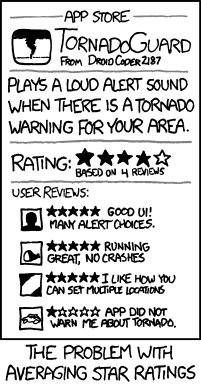
\includegraphics[width=\textwidth]{images/xkcd/tornadoguard.png}
  \captionof*{figure}{TornadoGuard \url{https://xkcd.com/937}}
  \label{fig:xkcd-tornadoguard}
\end{minipage}\hfill%
\begin{minipage}{.5\textwidth}
  \centering
  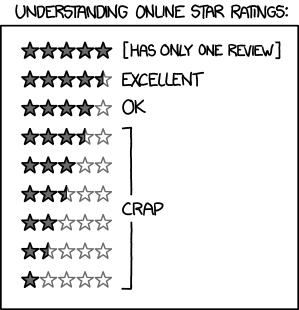
\includegraphics[width=\textwidth]{images/xkcd/star_ratings.png}
  \captionof*{figure}{Understanding online star ratings \url{https://xkcd.com/1098}}
  \label{fig:xkcd-star-ratings}
\end{minipage}
    \caption{XKCD's views on App Store Ratings and Reviews}
    \label{fig:xkcd-app-store-ratings}
\end{figure}
% https://www.explainxkcd.com/wiki/index.php/937:_TornadoGuard
% https://www.explainxkcd.com/wiki/index.php/1098:_Star_Ratings


Apps with poor ratings are less likely to be downloaded by new users~\sidecite{dimensionalresearch2015_mobile_app_use_and_abandonment}. Ratings also affect where an app appears in search results and whether an app store will choose to promote that app, or another. In the author's experience when one team's Android app's overall rating dropped from 4.4 to 4.3 stars the business noticed an almost immediate reduction in revenues from the app in addition to discovering that app was ranked lower in the search results. Therefore ratings are an important measure for app developers, and one they may choose to influence positively. 

Gaming ratings includes activities such as an app first asking if a user is happy with the app, and if they say yes then providing a link to encourage the user to rate the app positively in the app store. \textcite{novoda_akan2016_asking_for_app_feedback_the_effective_way} provides an illustrative industry case study of how Novoda improved the rating of a major newspaper's app. And in terms of the SDKs developers can use for in-app feedback, Apptentive is one of several companies that provides SDKs to help developers optimise their ratings and reviews and guides on how to do so within a mobile app~\sidecite{walz2015_apptentive_the_mobile_marketers_guide_to_app_store_ratings_and_reviews}. Unsurprisingly, ratings are also a subject of research interest.

Here are several representative papers that focus on engineering aspects of ratings and reviews.  \textcite{alsubaihin2019app_store_effects_on_software_engineering} discusses the symbiotic relationship between releases and the ratings and reviews that app received [p. 14]. Some developers time their releases based on the feedback they've received and monitor ratings and reviews for their latest release to influence the rollout of the new release. There have been innovative ideas on using ratings to prioritise software engineering activities including software testing of Android games apps~\sidecite{khalid2014_prioritizing_the_devices_to_test_your_app_on_casestudy_android_games}. And in \textcite{greenheld2018_automating_developers_responses_to_app_reviews} the value of developers responding to reviews was highlighted. 
In a population of 10,000 Android apps extracted from Google Play, correlations was identified between the density of warnings reported by FindBugs, a static analysis tool, and app store reviews and ratings for these apps~\sidecite{khalid2016_examining_the_relationship_between_findbugs_warnings_and_app_ratings}. They considered three warning categories: bad practices (which include reports of crashes in the reviews), internationalisation, and performance (which might relate to ANRs, however they didn't investigate this aspect). They did not investigate whether addressing warnings from FindBugs improved the ratings or reviews for those apps, and mobile analytics was not mentioned in their work - unsurprising as they took a black box approach using decompiled Android app binaries.

Via Figure \ref{fig:xkcd-app-store-ratings} XKCD aptly sums up two facets of flaws in app store ratings and reviews, averaging reviews may not be a good measure~\sidecite{explainxkcd_937_tornadoguard}, and the star ratings are not treated as a linear scale in practice~\sidecite{explainxkcd_1098_star_ratings}. In summary, app Store ratings therefore may not be an ideal measure of the quality of an app from a software engineering perspective! 
% See also stanik2020_requirements_intelligence_on_the_analysis_of_user_feedback
% shen2017_towards_release_strategy_optimization_for_apps_in_google_play 

\subsection{Reviews in app stores}
Similarly reviews in app stores have been analysed for various purposes including for complaints and bug reports. Of the many and various research on reviews of mobile apps in app stores. 
Two early papers, the first focusing on Android apps in Google Play~\textcite{fu2013_why_people_hate_your_app_making_sense_of_user_feedback_in_a_mobile_app_store} and the second for iOS apps in Apple's App Store~\textcite{khalid2015_what_do_mobile_app_users_complain_about}.

In \textcite[p. 5][]{fu2013_why_people_hate_your_app_making_sense_of_user_feedback_in_a_mobile_app_store} the top three most common indicators of problems in the apps were: slow 9,939, crashes 9,081, and freezes 3,960. Stability was a common theme of complaints about both free and paid apps [pp. 7-9]. 

In \textcite{khalid2015_what_do_mobile_app_users_complain_about} clearly establishes connections between what users of iOS apps complain about and the effects of these complaints on ratings of those apps; and \textcite{panichella2015_how_can_i_improve_my_app_classifying_user_reviews_for_sw_maintenance_and_evolution} extends that work to consider the relevance of various review-topics to developers. Panichella \emph{et al} also extend the work to include Android apps in the Google Play Store. \textcite{mcilroy2016_analyzing_and_automatically_labelling_the_types_of_user_issues_raised_in_mobile_app_reviews} - labels the content of reviews extracted from Google Play and found crashes and crashing were one of the topics that was a) relatively easy to categorise, and b) occurred frequently. This paper seemed to conflate in-app analytics tools (Flurry) with analytics of reviews (e.g. AppAnnie). As an observation, since this paper was published Google Play now provides automated labeling and analysis of reviews.

Feedback comes in various forms, ratings and reviews are only two of them.  One that's seldom used in industry and seldom researched is implicit feedback recorded through user-interactions with the GUI of the mobile app. Common terms for this mechanism include `heatmaps' and `heatmapping' and there are commercial SDKs and opensource projects available that perform the recording within an app at runtime. The elixir of automating `record and playback' test automation sometimes uses similar methods to record the interactions with a mobile app. 

\subsection{Testing}
\emph{``How do Developers Test Android Applications?"}~\sidecite{linares2017_how_do_developers_test_android_apps}. Quote:~\emph{``“I mostly do manual testing due to the limited size of my apps. I sometimes use a custom replay system (built into the app) to duplicate bugs after I come across them. This method is usually combined with manual testing (printing debug information to the log) to pinpoint the cause”."}

The absence of automated tests does not prove developers do not test their Android apps, rather it indicates their projects are unlikely to have any automated tests and similarly that the project is unlikely to run any automated scripted tests as part of a continuous build. (In honour of Dijkstra's observation that ``Testing shows the presence, not the absence of bugs'', Edsger W. Dijkstra in ~\textcite[p. 16][]{randell1970_software_engineering_techniques_nato_dijkstra}.) % Found via https://en.wikiquote.org/wiki/Edsger_W._Dijkstra
% See also: https://www.techwell.com/techwell-insights/2018/12/can-we-ever-find-all-bugs 
% https://wiki.c2.com/?TestsCantProveTheAbsenceOfBugs

An incredible amount of research energy has gone into trying to find better ways to test mobile apps, ranging from autonomous tools that where the researchers endeavour to deliver better coverage than a small free utility called \texttt{monkey} (and sometimes manage to do so), through to ways to generate automated tests from the text of reviews. Virtually none of these endeavours seem to make any difference to the testing developers do, they don't use the tools developed from these research efforts. 

\emph{``Thus even if the app is tested on one device, there is no guarantee that it may work on another device."}~\cite[p. 27]{nagappan2016_future_trends_in_sw_eng_for_mobile_apps} - I agree. They don't provide any substance for this statement.

research gaps...

And yet, researchers also continue to complain app developers don't test their apps sufficiently. They sometimes berate the app developers to `test their apps' ,\emph{e.g.}~\textcite{cruz2019_guess_what_test_your_app}.
Similarly the voices of the researchers seem to go unacknowledged and unapplied.

Another strand is where researchers collate examples of apps together with faults they have identified and analysed in order to help, primarily, other researchers. 

Why are all these efforts to improve software testing for mobile apps generating seemingly minimal effects in practice? Perhaps researchers into improving mobile apps would find an approach similar to the research of~\textcite{winter2022_lets_talk_with_developers_etc_automatic_program_repair} more productive - by actually talking \emph{with} the app developers and then offering to research pain points identified by those app developers. Doing so might increase the external and ecological validity of the research and potentially also increase the adoption of the research. The adoption might be at an individual developer, team, or organisation level. In some instances the effects of the research may gain wider adoption and become a tool, technique, approach that many app developers adopt. In some cases the app store and/or platform provider might also adopt the work, for instance to replace their current `monkey' test tool. As an aside Google already has replaced their `monkey' utility with `robo'.

Developers do want automated tests and tools to provide them with feedback~\cite[p. 5]{greiler2022_an_actionable_framework_for_understanding_and_improving_developer_experience} even if relatively few projects have sufficient tests to provide the developers with a level of comfort and confidence. Again, much of the research has focused on where researchers can find tests rather than working with development teams to understand their desires and the barriers that mean the developers don't have (m)any tests. 

For project teams with large volumes of automated tests, what value do those tests provide? Fortuitously one of the app-centric case studies, Catrobat, has an opensource codebase and their uses of automated tests are well researched. The Catrobat project makes extensive use of various forms of automated tests including using Behaviour-Driven-Development (BDD) practices~\textcite{ali2019using_catrobat}, testing under adverse conditions~\textcite{adamsen2015systematic_catrobat}, the use of sizing for automated tests~\textcite{hirsch2019approach_catrobat}, \emph{etc}. % TODO add additional references for Catrobat. See the findings-results chapter.

\subsection{Mobile Analytics}
In-app analytics have been used to help developers understand ways their mobile app is used by large populations of end-users and the effects of various conditions on the behaviours of the end users. There has been some research into using mobile analytics to understand usage patterns of specific apps, for example:

\begin{itemize}
    \item \textcite{parate2016_RECKON_an_analytics_framework_for_app_developers_HP_AppPulseMobile} describes how automatic instrumentation of mobile apps using mobile analytics tools including HP's App Pulse Mobile is able to help developers better understand their users.
    \item \textcite{ferre2017_extending_mobile_app_analytics_for_usability_test_logging} identified the importance of usability testing in terms of success of mobile apps, while there are challenges and severe limitations with usability testing in the lab. This research evaluated the use of Google Analytics for Mobile Applications to provide continuous usability logging. They describe a three-stage proposed approach to logging. In the third stage they have two alternatives, one for lab usability testing, the other for continuous usability logging.
    \item and the Insight toolkit~\textcite{patro2013_capturing_mobile_experience_in_the_wild} which is covered in more detail next.
\end{itemize}   

Two mobile apps incorporated a toolkit library called Insight~\cite[p. 82]{patro2015_building_blocks_to_understand_wireless_experience}~\footnote{Interim aspects of this research was also published~\textcite{patro2013_capturing_mobile_experience_in_the_wild}.} that combined passive analytics, such as session length, with factors, such as network condition and client device, with the aim of helping the developers recognise correlations between these factors and application use and revenues[p. 82](\textit{ibid}).

The research describes generic data, collected by Insight for any app, and app-specific data, which is defined and implemented by the developers of that app~\cite[pp. 87-88]{patro2015_building_blocks_to_understand_wireless_experience}. They identified a correlation between battery drain and session lengths, as battery drain increased the session lengths decreased, and also the correlation between screen brightness and battery drain. The device model was a material factor in the rate the battery drained, and in particular on Kindle Fire devices the drain was far higher when the screen was bright. ``\emph{controlling the screen brightness on a Kindle Fire device reduced the average battery drain by 40\% while using SB}''~\cite[p. 13]{patro2015_building_blocks_to_understand_wireless_experience} Note: SB is short for StudyBlue, one of the two apps in this study.

The research using Insight was one of the catalytic agents for this research as it was able to publish data obtained using mobile analytics for two popular real-world apps. They also made both their client and server code freely available online as opensource projects: \url{https://github.com/patroashish/InsightClient} and \url{https://github.com/patroashish/InsightServers}. Although they mention they developed an iOS SDK it does not appear to have been made available online~\cite[p. 85]{patro2015_building_blocks_to_understand_wireless_experience}.

Perhaps paradoxically the Insight client SDK, freely available at \url{https://github.com/patroashish/InsightClient}, does not record or report any failures of the SDK or of the associated app it has been integrated with. Assuming crashes, freezes, and other similar issues might affect the end-user experience it seems odd the SDK doesn't track these aspects. Furthermore the SDK only sends the analytics data when there is a working mobile network immediately available, it does not appear to queue events, incorporate any robustness mechanisms, or include any re-transmission capabilities.

With the exception of a brief comparison between Insight and three then popular mobile analytics services their research does not investigate any other mobile analytics offering.

Note: there has also been research into similar sounding work on software analytics for mobile apps~\textcite{minelli2013_software_analytics_samoa}, however that research is into characteristics of the source code rather than in the use of mobile analytics by app developers.

Research into mobile analytics is surprisingly rare, especially given the prevalence of apps that include mobile analytics SDKs and their use by mobile app developers. A possible reason for the rarity is the challenges in researchers obtaining access to the outputs of the mobile analytics. For the research using Insight they negotiated special non-disclosure agreements (NDAs) and the data was pre-filtered to increase the privacy of the end users~\cite[p. 91]{patro2015_building_blocks_to_understand_wireless_experience}. 

Before we leave the topic of mobile analytics research into the privacy aspects of the mobile analytics SDKs is pertinent as the choices developers make in terms of selecting in-app mobile analytics has various consequences including the privacy for the end users who indirectly provide the underlying data. Two illustrative areas of research into the privacy and data leakage aspects are:

\begin{itemize}
        \item \textcite{razaghpanah2018_apps_trackers_privacy_and_regulators_a_global_study_of_the_mobile_tracking_ecosystem} where a privacy-focused app is used to obtain the network traffic sent to ad and analytics end points from end-user devices. That traffic is analysed to understand where it goes, who has access to the underlying data, and what of the content is most likely to contravene ePrivacy and GDPR directives.
        \item \textcite{liu2020_privacy_risk_analysis_and_mitigation_of_analytics_libraries_in_the_android_ecosystem}, in contrast, modifies the binary files of various apps in order to intercept the calls to the respective in-app SDKs of various mobile analytics libraries. They developed a proof-of-concept Android app AlManager that a) allows the user to see the contents of the calls made to the in-app SDKs, and b) to block or replace the contents with blank data. They also studied characteristics of the calls the apps made in terms of the App, Activity, and User level in terms of the data being sent to the mobile analytics SDK(s).
\end{itemize}

The first of these papers focuses on the data that is sent, the contents, and where that data goes. The second concentrates on analysing app binaries, finding all the calls to the mobile analytics SDKs, intercepting these and enabling users to see, block or blank out data that would then be sent by the respective mobile analytics SDK.


\section{Mobile App Crashes}~\label{rw-mobile-app-crashes-topic}
Crashes in mobile apps have garnered a great deal of research, perhaps as crashes are definitive and relatively easy to detect.

There is some interesting large-scale research into analysis of various releases of production Android application binaries~\sidecite{kong2019_mining_android_crash_fixes}. The researchers exercised (tested) a large range of apps seeking crashes of the app using an oracle of a local log file which they queried using the standard Android \texttt{logcat} utility. They also combined their dynamic approach with using static analysis tools to identify potential flaws that would lead to crashes of an app. They then tested newer releases of the same app. If the newer version did not crash they analysed the binary files (the APK files) for both releases to differences to the compiled code that may have been responsible for 'fixing' the crash. They limited their work to Android \emph{framework specific} crashes, and excluded \emph{app-specific} crashes. They devised ways to identify changes that appeared to fix the particular crash(es) they triggered in the earlier releases and generated patch files based on these changes. These patches were then applied to the older release of the app and the app then tested with the same test inputs and runtime environment (at least in terms of using a consistent Android Emulator (also known as a virtual device)). They provide a relatively detailed replication package online at~\url{https://craftdroid.github.io/}.

\begin{itemize}
    \item Their approach is innovative and could help real-world developers of Android apps to identify and apply snippets of code to reduce the likelihood of their app suffering the same crash. Their 17~\href{https://github.com/CraftDroid/ExpData/tree/master/Fix_Templates}{fix templates} act as guides for Android developers and could potentially be implemented into code-quality tools.
    \item However it only applied for framework specific crashes, and their choice of runtime environment meant they could only install 56\% of the APKs. There are many other sources of crashes, and also apps that include native code (several of my case study apps do). Also their testing is limited to automated `monkey' testing which may further limit the crashes their approach can find in production apps, particularly those that incorporate user accounts, user-specific content, behaviour, online purchases and many other forms of activities.
    \item The supporting website \url{https://github.com/CraftDroid} includes scripts and log extracts for the crash reproductions, it lacks the mechanisms for generating diffs, applying them, or building the patched APK. The lack of these mechanisms makes the efficacy of their approach hard to reproduce.
    \item It also does not appear to test for crashes related to third-party libraries e.g. OkHttp which is extremely popular in Android apps; however potentially this approach could be extended to do so?
\end{itemize}

In summary, the approach proposed in~\sidecite{kong2019_mining_android_crash_fixes} has the potential to mine crash stack traces (which are available to the developers of the particular apps) to help with aspects of reproducing a subset of those crashes which pertain to Android framework-related crashes. Similarly it appears it could complement the automated testing provided by Google as part of the pre-launch reports available in Google Play Console and other services. 

In contrast, ~\sidecite{wang2018_an_empirical_study_of_android_test_generation_tools_in_industrial_cases} evaluated a mixed set of industrial and opensource test automation tools against popular Android apps available in Google Play. They measured code coverage and the count of unique crashes each tool could find in these apps. They also considered more practical aspects such as finding ways to combine tools to increase the code coverage and fault detection, they also measured the effort required to setup each of the tools to test the industrial apps. Their reference tool was Android `Monkey' the ubiquitous tool shipped with the Android SDK and one of the most widely used of these tools. This research appears practical and well grounded. It does not compare any aspect of crashes in the wild \emph{i.e.} those that affect end users and some of the crashes that were detected, such as those reported when Sapienz was used to test the Wattpad app might have established sufficiently unusual conditions for those crashes to be unlikely for most end users. (Nonetheless these crashes might still be of interest to the app's developers). 

The authors did not mention whether they reported the crashes to the app developers, which is a pity as it would have been interesting to learn whether the app developers were willing and able to fix the crashes. If the researchers had reported the crashes to the app developers then this research - if combined with the research in the previous paper~\sidecite{kong2019_mining_android_crash_fixes} - could have been enlightening to measure at a black box level whether the crashes had been successfully fixed post reporting them.


\section{Summary so far} % Or curiosities, or gaps in the research at this stage...?
App stores, their ecosystems, and their effects on developers have been covered from various angles. Some of the research describes snapshots of one or more app stores. And some of the research involves developers of live apps in a mainstream app store. Ratings and reviews are covered from many angles including fraud~\sidecite{xie2015_appwatcher_unveiling_the_underground_market_of_trading_mobile_app_reviews}. 

One of the curiosities reported in~\textcite{alsubaihin2019app_store_effects_on_software_engineering} is: \emph{``while automatic in-app crash reporting is the most prolific channel of reporting bugs, the one mostly prioritised by our respondents is user reviews in app stores."}[p. 13] - what are the effects of the crashes being a lower priority than user reviews? Also, they don't discuss other sources of crash reports (e.g. platform crash reporting) even though these existed at the time of their research.

Similarly, in terms of managing releases in app stores, the platform provided release management tools and reports were not mentioned. 

Several points made in \sidecite{frankl1997choosing_testing_for_reliability} discuss the potential perils of relying on the judgement of people involved in debug testing (testing to maximise the faults found in a given period), the first point is based on work by \sidecite{basili1994_software_process_evolution_at_the_sei} where testers who focused on `testing' over estimated their abilities to find all the faults in a program, by proposing it is possible to compare the effectiveness of testing by using operational profiles~\sidecite[][p. 77]{frankl1997choosing_testing_for_reliability}.

The second point is there is the potential for debug testers to confuse \emph{``between detecting failures and achieving reliability.''}~\sidecite[][p. 77]{frankl1997choosing_testing_for_reliability}. Mobile Analytics might be able to provide a real-world measure in terms of achieving reliability. Furthermore, much of the research into mobile app crashes seems to end prematurely - before considering whether reliability of the app has been improved by whatever method and approach they have researched.

\begin{quote}
    \emph{``...with explicit and implicit feedback now available (almost) continuously, questions arise. How can practitioners use this information and integrate it into their development processes to decide when to release updates?''}\cite[pp. 48-49]{maalej2016_towards_data_driven_requirements_engineering}    
\end{quote}

Building on a point made in this paper: \emph{``the future of app quality engineering is data driven."}~\cite[p. 24]{nagappan2016_future_trends_in_sw_eng_for_mobile_apps} % cite 97.


\julian{TODO complete this thought: However none of these (these researches) provide X which is my need...}